\documentclass[handout,compress]{beamer}

\usetheme[block=fill]{metropolis}

\usepackage{graphicx} % Allows including images
\usepackage{amsmath,amsfonts,amsthm,amssymb}
\usepackage{color}
\usepackage{xcolor,cancel}
%\setitemize{label=\usebeamerfont*{itemize item}%
%	\usebeamercolor[fg]{itemize item}
%	\usebeamertemplate{itemize item}}
\definecolor{mDarkBrown}{HTML}{604c38}
\definecolor{mDarkTeal}{HTML}{23373b}
\definecolor{mLightBrown}{HTML}{EB811B}
\definecolor{mMediumBrown}{HTML}{C87A2F}
\definecolor{mygreen}{HTML}{98C2B9}
\definecolor{myyellow}{HTML}{DFD79C}
\definecolor{myblue}{HTML}{8CA7CC}
\definecolor{kern}{HTML}{8CC2B7}

\usepackage{float}
\usepackage{framed}
\usepackage{epsfig}
\usepackage{graphicx}
\usepackage{subcaption}
\usepackage{ulem}
\usepackage{hhline}
\usepackage{multirow}
\usepackage{comment}   
\usepackage{bbm}
\usepackage{tikz}   
\usepackage{ulem}
\def\Put(#1,#2)#3{\leavevmode\makebox(0,0){\put(#1,#2){#3}}}
\newcommand*\mystrut[1]{\vrule width0pt height0pt depth#1\relax}
\newcommand{\eqdef}{\mathbin{\stackrel{\rm def}{=}}}


\newcommand{\bs}[1]{\boldsymbol{#1}}
\newcommand{\bv}[1]{\mathbf{#1}}
\newcommand{\R}{\mathbb{R}}
\newcommand{\E}{\mathbb{E}}

\DeclareMathOperator*{\argmin}{arg\,min}
\DeclareMathOperator*{\argmax}{arg\,max}
\DeclareMathOperator{\nnz}{nnz}
\DeclareMathOperator{\Var}{Var}
\DeclareMathOperator{\sinc}{sinc}
\DeclareMathOperator{\mv}{mv}
\DeclareMathOperator{\sgn}{sgn}
\DeclareMathOperator{\step}{step}
\DeclareMathOperator{\gap}{gap}
\DeclareMathOperator{\poly}{poly}
\DeclareMathOperator{\tr}{tr}
\DeclareMathOperator{\orth}{orth}
\newcommand{\norm}[1]{\|#1\|}
\captionsetup[subfigure]{labelformat=empty}
\captionsetup[figure]{labelformat=empty}
\DeclareMathOperator*{\lmin}{\lambda_{min}}
\DeclareMathOperator*{\lmax}{\lambda_{max}}

\newcommand{\specialcell}[2][c]{%
	\begin{tabular}[#1]{@{}c@{}}#2\end{tabular}}
\newcommand{\specialcellleft}[2][c]{%
	\begin{tabular}[#1]{@{}l@{}}#2\end{tabular}
}

\usepackage{tabstackengine}
\stackMath

\newtheorem{claim}[theorem]{Claim}


%----------------------------------------------------------------------------------------
%	TITLE PAGE
%----------------------------------------------------------------------------------------

\title{CS-UY 4563: Lecture 19 \\ Convolutional Neural Networks}
\author{NYU Tandon School of Engineering, Prof. Christopher Musco}
\date{}

\begin{document}
	
	\begin{frame}
		\titlepage 
	\end{frame}
	
	\metroset{titleformat=smallcaps}
	
	\begin{frame}
		\frametitle{course logistics}
		\begin{itemize}
			\item I will be reviewing project proposals over the next few days. If you need feedback sooner, please email separately to set up a meeting, or stop by office hours.
			\item Written Homework 4 due \textbf{next Monday}.
			\item Work through \texttt{demo\_convolutions.ipynb}, now on course website.
		\end{itemize}
	\end{frame}

	\begin{frame}
	\frametitle{convolutional feature extraction}
	\textbf{Last lecture:} \alert{\textbf{Convolution}} in 1, 2, and 3D is a powerful generic tool for designing natural \textbf{feature transformations} for time-series data, audio data, or images.
	\begin{center}
		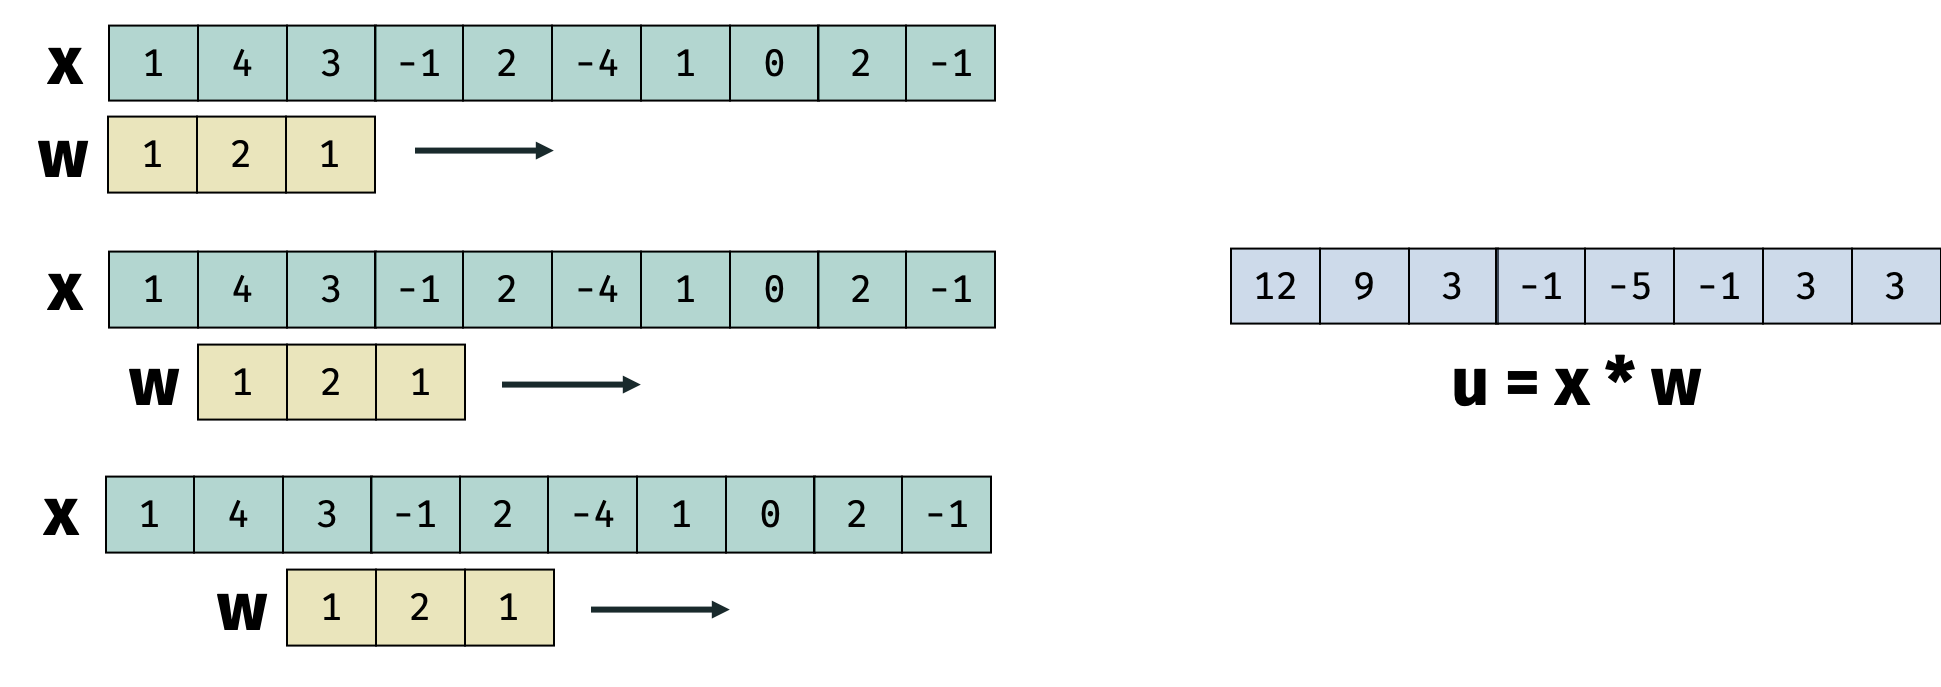
\includegraphics[width=.9\textwidth]{compact_conv.png}
	\end{center}
	\end{frame}

	\begin{frame}
	\frametitle{2d convolution}
	\small\centering
	$\bv{w} = \begin{bmatrix}0&1&2\\2&2&0\\0&1&2\end{bmatrix}$ 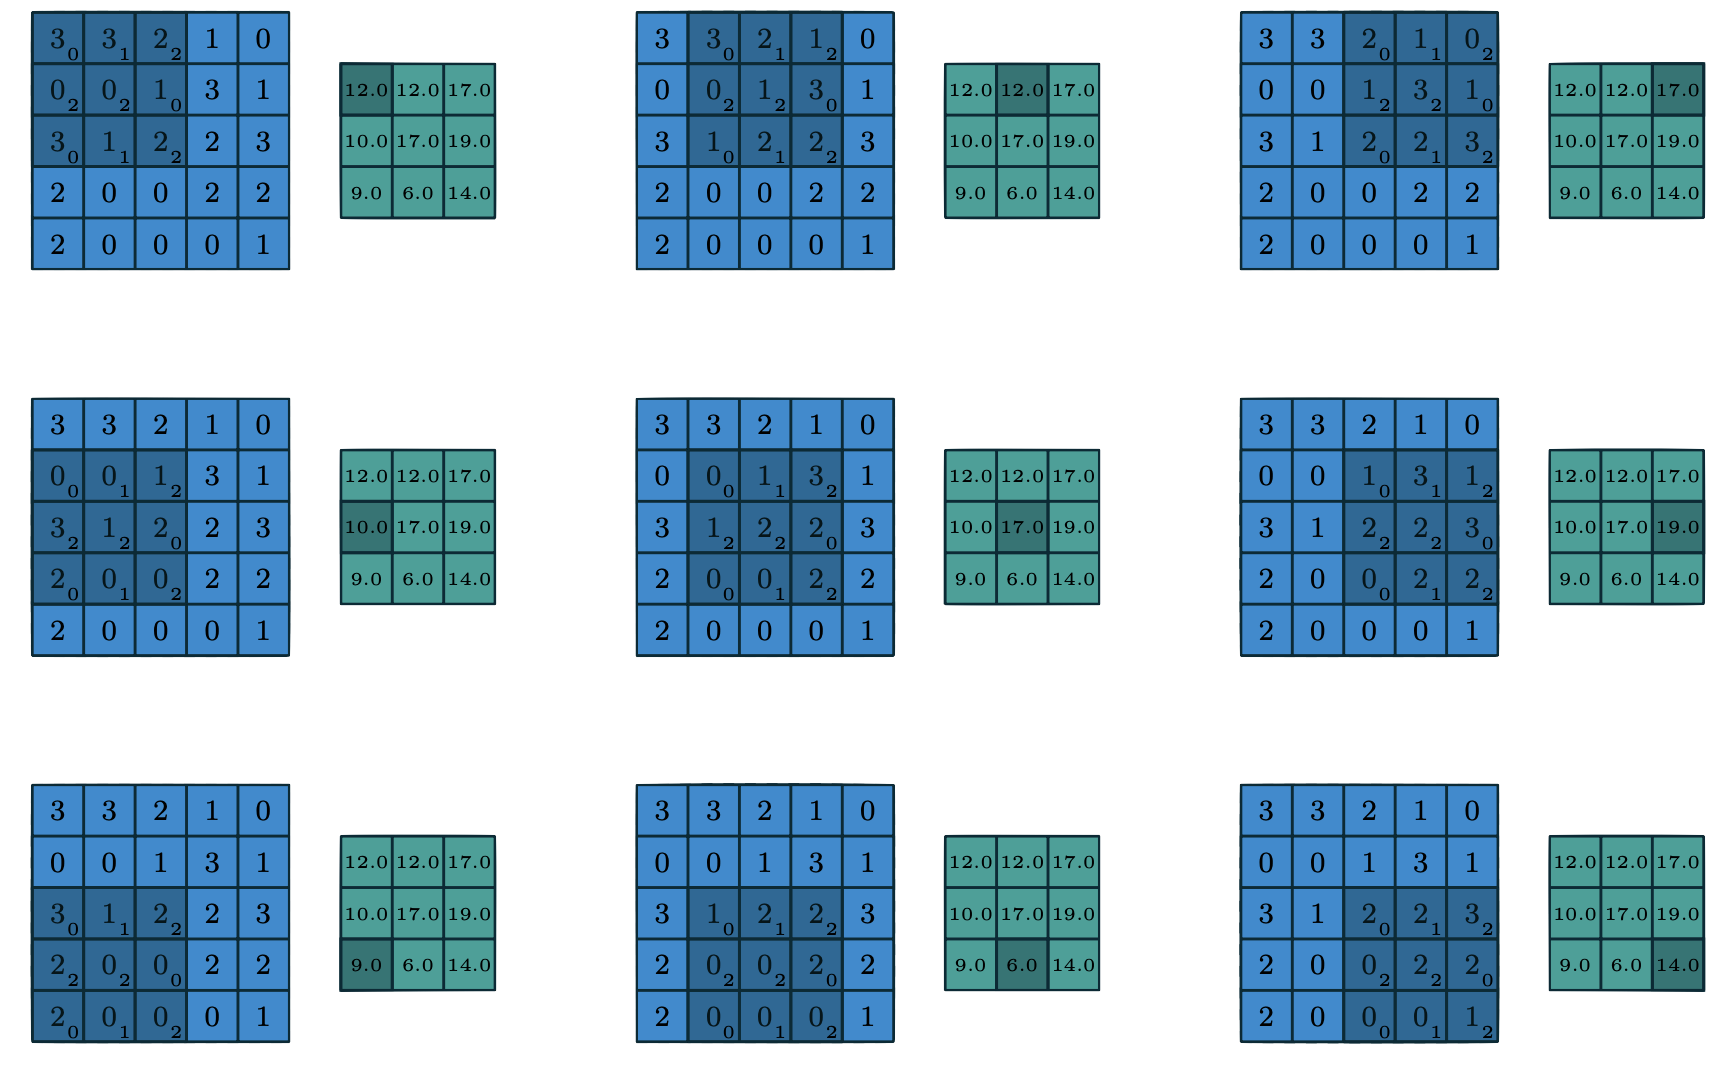
\includegraphics[width=.9\textwidth]{standard2d.png}
	\end{frame}

	\begin{frame}
		\frametitle{application 1: smoothing}
		A uniform or Gaussian filter can be used to smooth input data:
			\begin{center}
			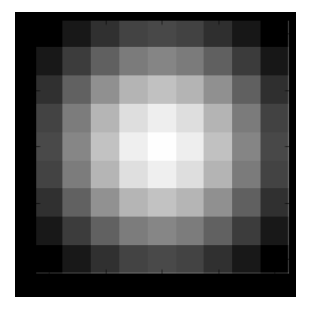
\includegraphics[width=.2\textwidth]{gaussian_filter.png}
			
			
			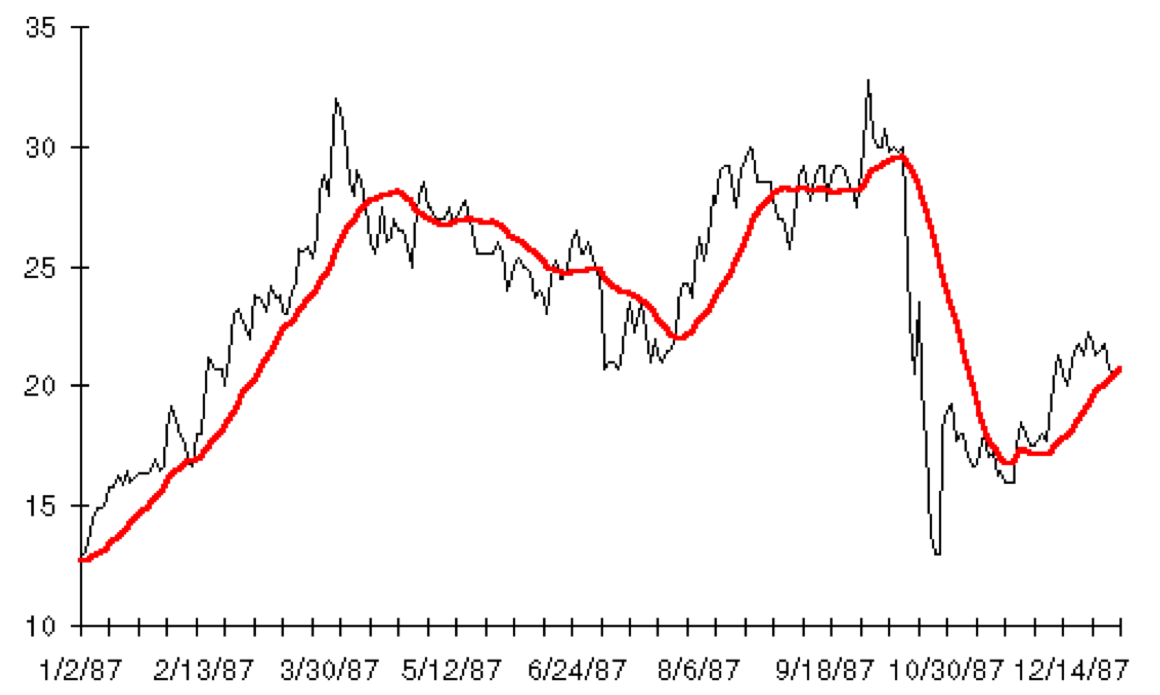
\includegraphics[width=.4\textwidth]{smoothtime_series.png}~ \includegraphics[width=.5\textwidth]{uniform_only.png}
		\end{center}
	\end{frame} 

	\begin{frame}
	\frametitle{application 2: pattern matching}
	Convolution can be used to find local patterns in images:
	\begin{center}
		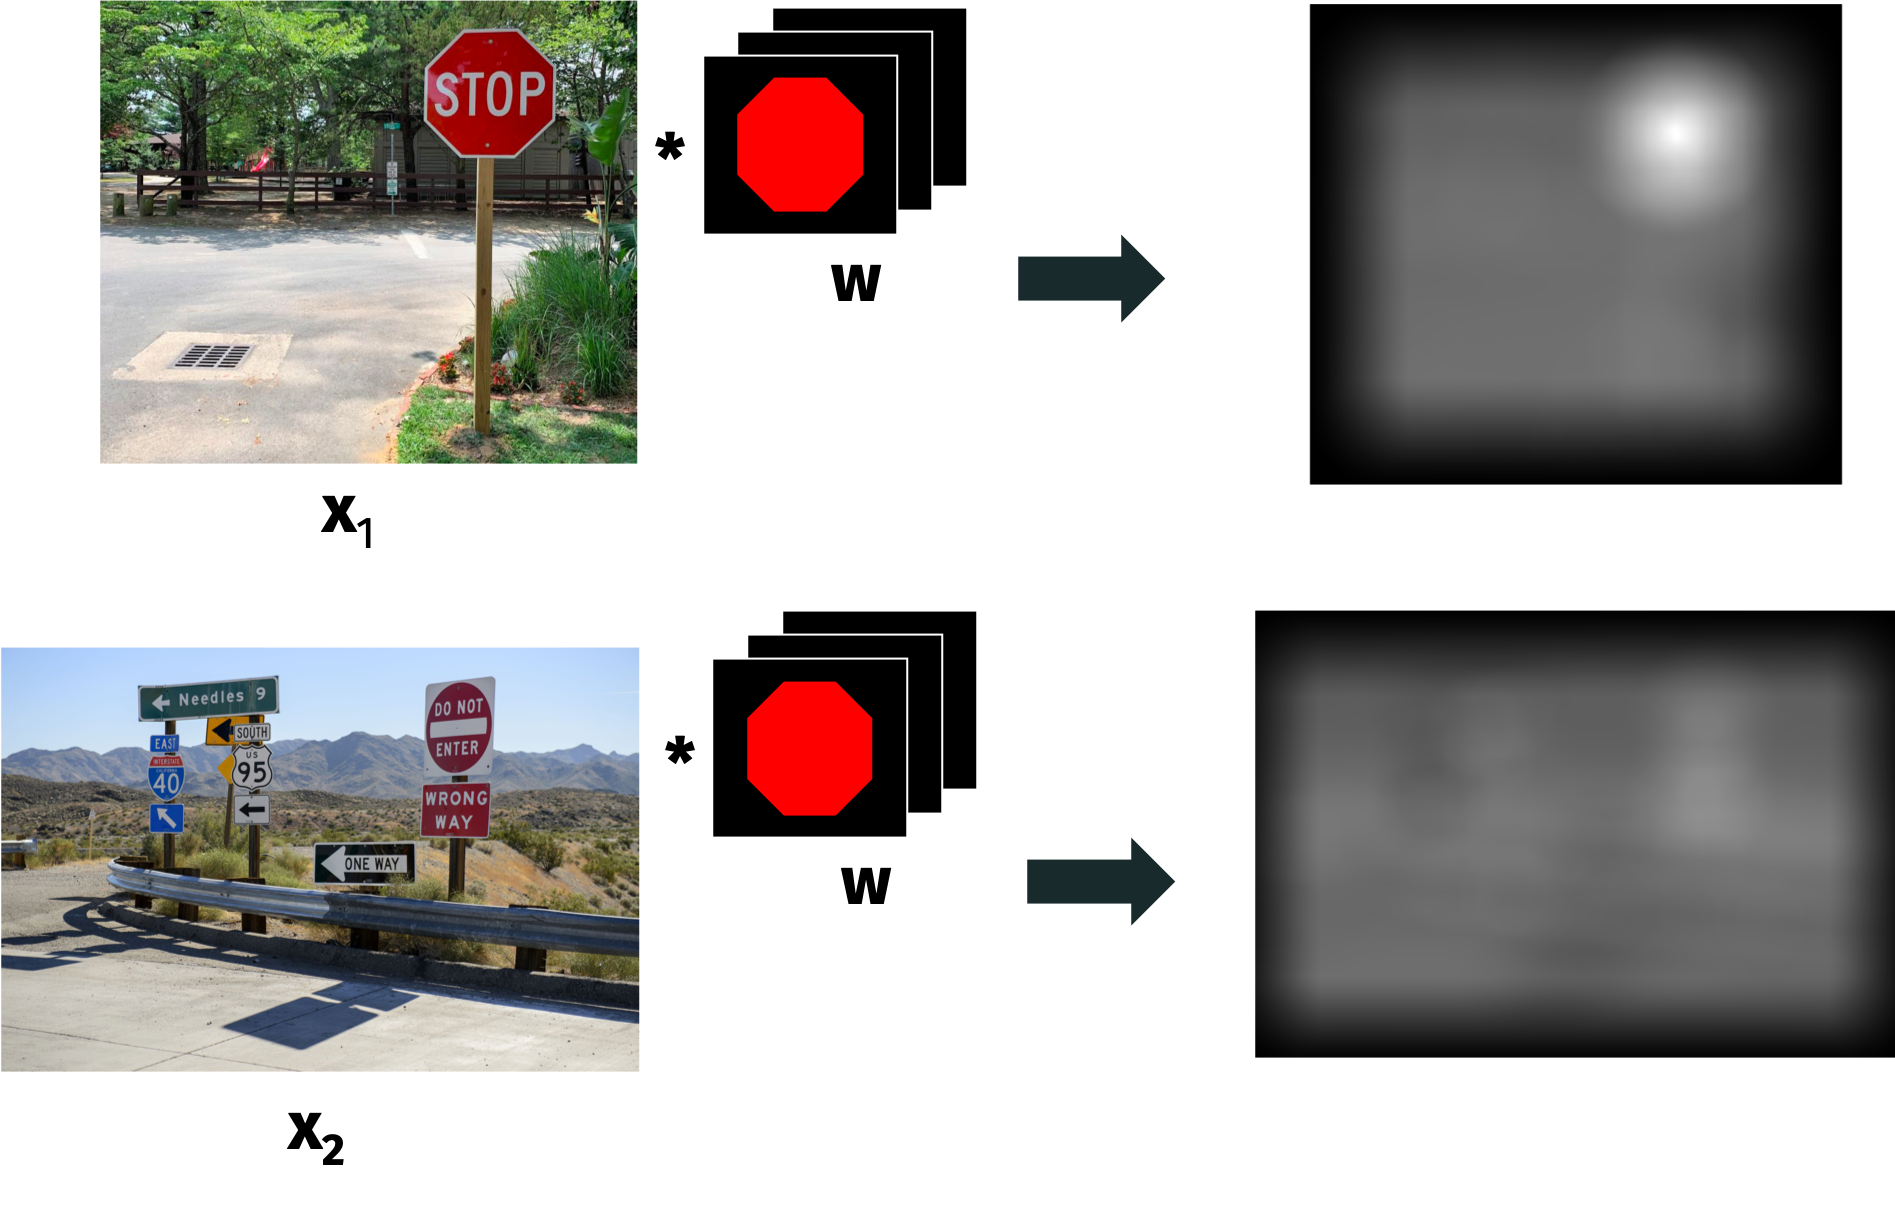
\includegraphics[width=.8\textwidth]{pattern_match.png}
	\end{center}
\end{frame} 

	\begin{frame}
	\frametitle{side note}
	\textbf{Good question from Piazza:} Won't this filter yield lots of false positives?
	\begin{center}
		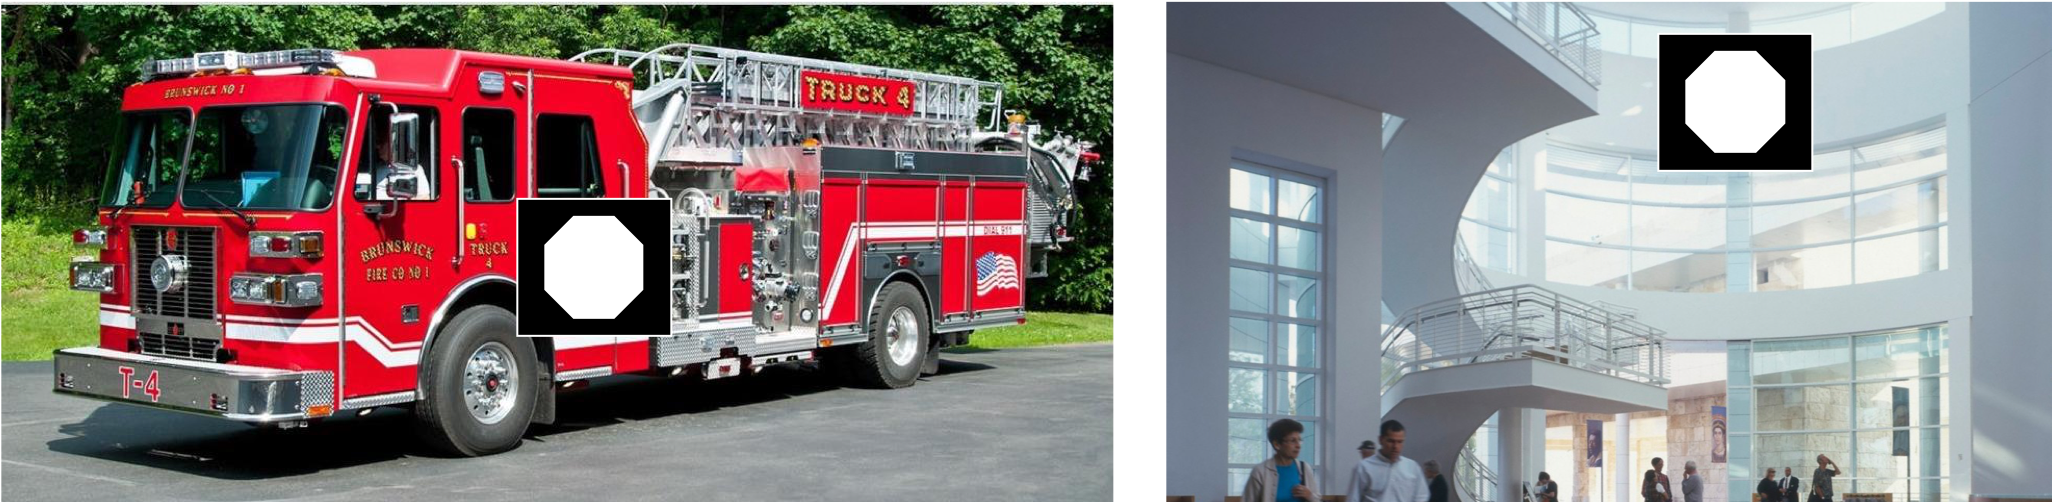
\includegraphics[width=.8\textwidth]{false_positive.png}
	\end{center}
	\end{frame}


\begin{frame}
	\frametitle{side note}
	\textbf{Possible fix that doesn't require image normalization:}
	\begin{center}
		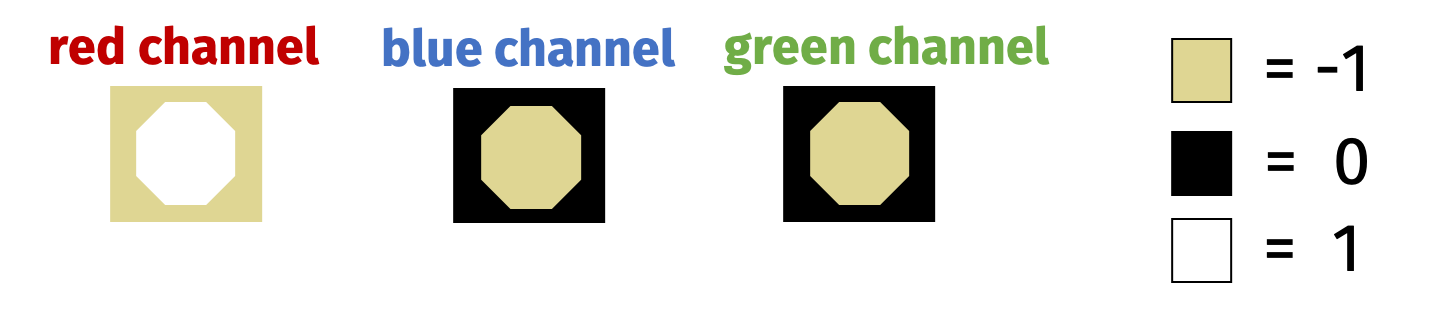
\includegraphics[width=.8\textwidth]{ying_fix.png}
	\end{center}
\end{frame}

\begin{frame}
	\frametitle{applications of convolution}
	\small
	\textbf{Application 3:} Edge detection.
	
	Consider a 2D \emph{edge detection filter:}
	\begin{align*}
	W_1 &= \begin{bmatrix}
	1 & -1
	\end{bmatrix} & 	
	W_2 &= \begin{bmatrix}
	1\\
	-1
	\end{bmatrix}
	\end{align*}
	\begin{center}
		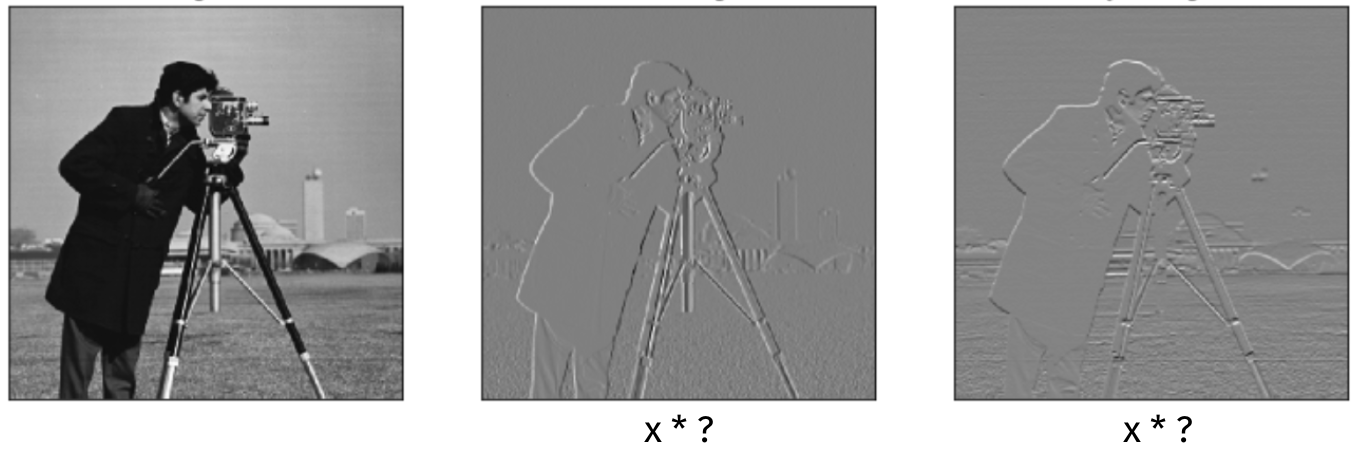
\includegraphics[width=\textwidth]{conv_test.png}
	\end{center}
\end{frame}

\begin{frame}
	\frametitle{applications of convolution}
	\textbf{Sobel} filter is more commonly used:
	\begin{align*}
	W_1 &= \begin{bmatrix}
	1 & 0 & -1\\
	2 & 0 & -2\\
	1 & 0 & -1
	\end{bmatrix} & 	
	W_2 &= \begin{bmatrix}
	1 & 2 & 1\\
	0 & 0 & 0\\
	-1 & -2 & -1
	\end{bmatrix}
	\end{align*}
	\begin{center}
		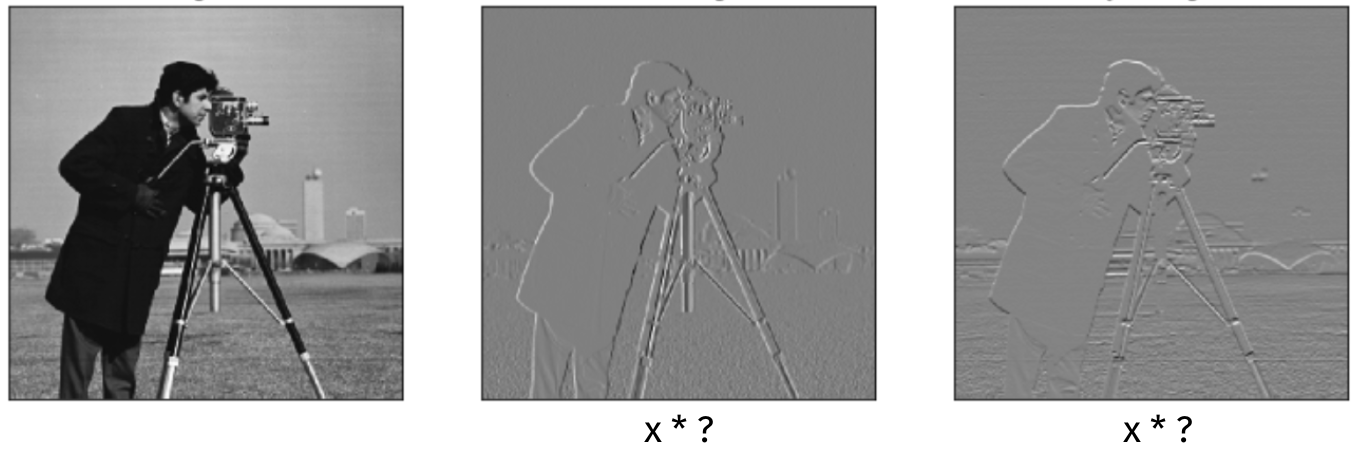
\includegraphics[width=\textwidth]{conv_test.png}
	\end{center}
\end{frame}

\begin{frame}
	\frametitle{directional edge detection}
	Can define edge detection filters for any orientation.
	\begin{center}
		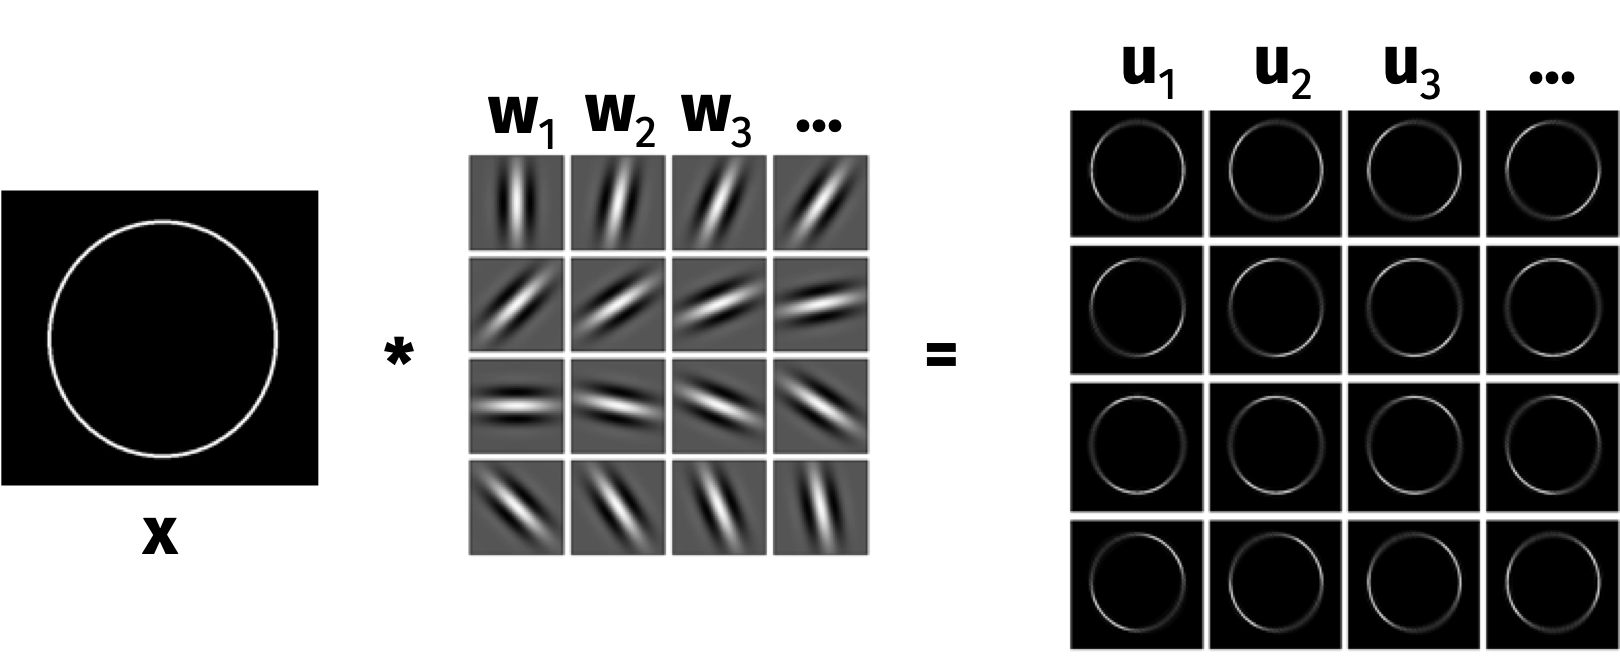
\includegraphics[width=\textwidth]{directional_edge.png}
	\end{center}
\end{frame}

\begin{frame}
	\frametitle{edge detection}
	How would edge detection as a \emph{feature extractor} help you classify images of city-scapes vs. images of landscapes?
	\begin{center}
		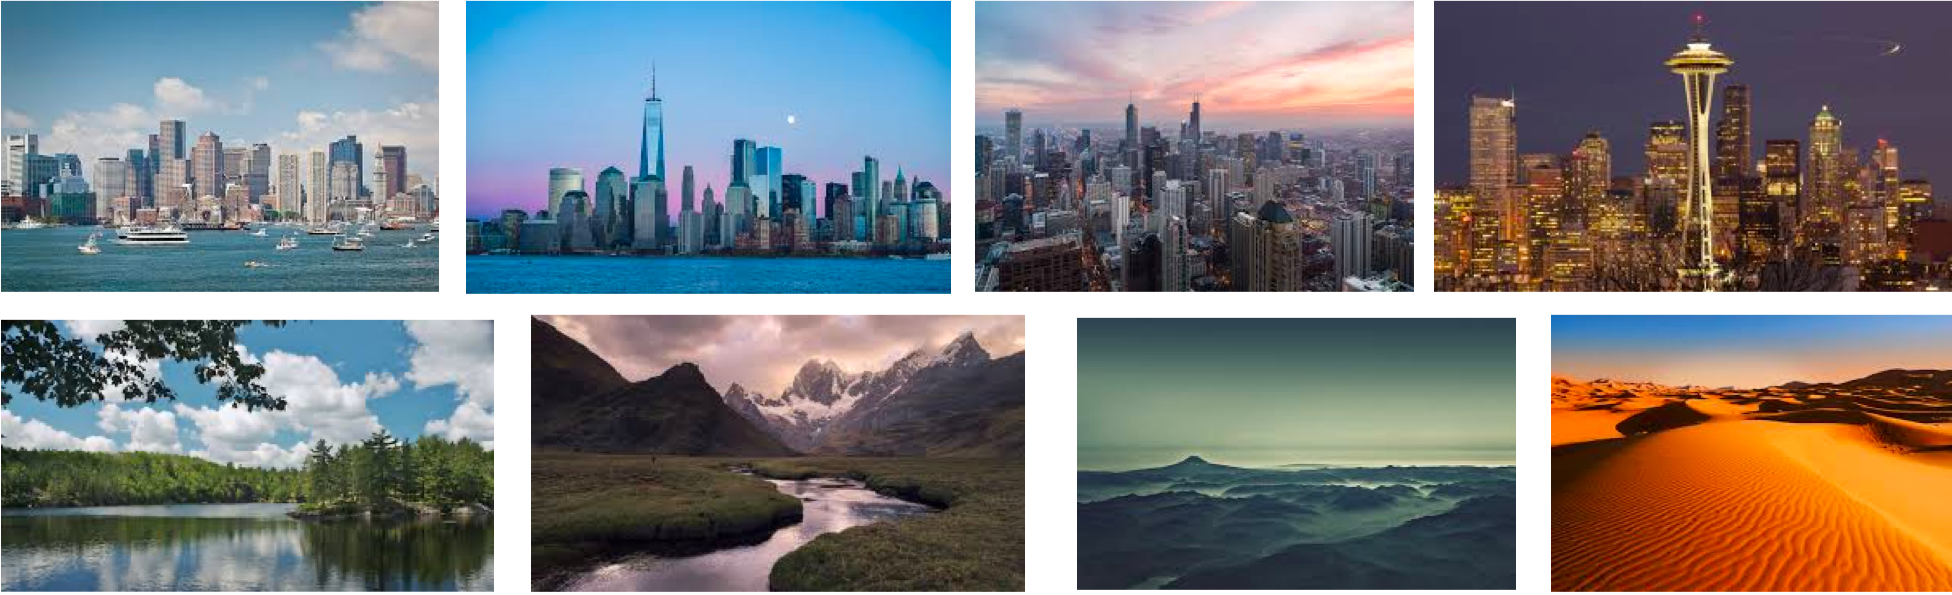
\includegraphics[width=\textwidth]{scapes.png}
	\end{center}
\end{frame}


\begin{frame}
	\small
	\frametitle{edge detection}
	\begin{center}
	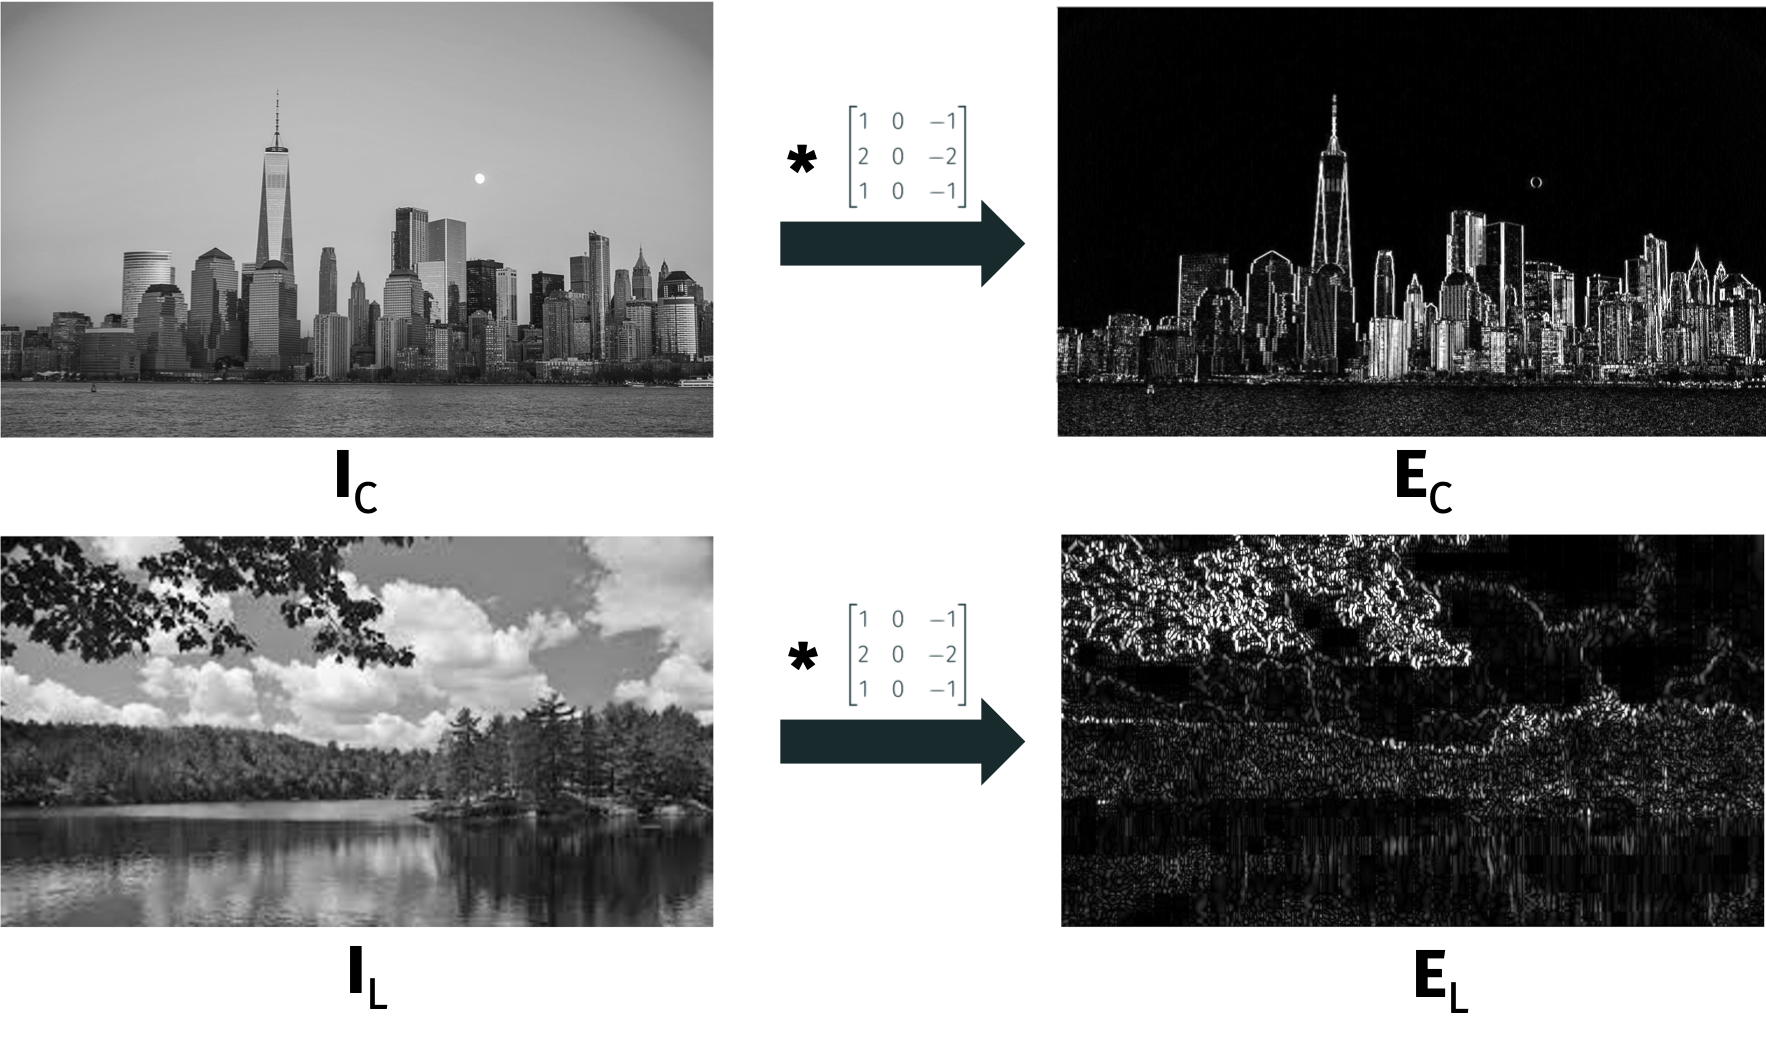
\includegraphics[width=.9\textwidth]{scape_edge.png}
	
	$\texttt{mean}(\bv{I}_C) = .108$ \hspace{1em} vs. \hspace{1em} $\texttt{mean}(\bv{I}_L) = .123$
	\end{center}
The image with highest vertical edge response isn't the city-scape.
\end{frame}

\begin{frame}
	\frametitle{edge detection + pattern matching}
	Feed edge detection result into pattern matcher that looks for long vertical lines.
	\begin{center}
		\includegraphics[width=.9\textwidth]{level2}
		
	\end{center}
\end{frame}

\begin{frame}
	\frametitle{hierarchical convolutional features}
	\small
	\begin{center}
	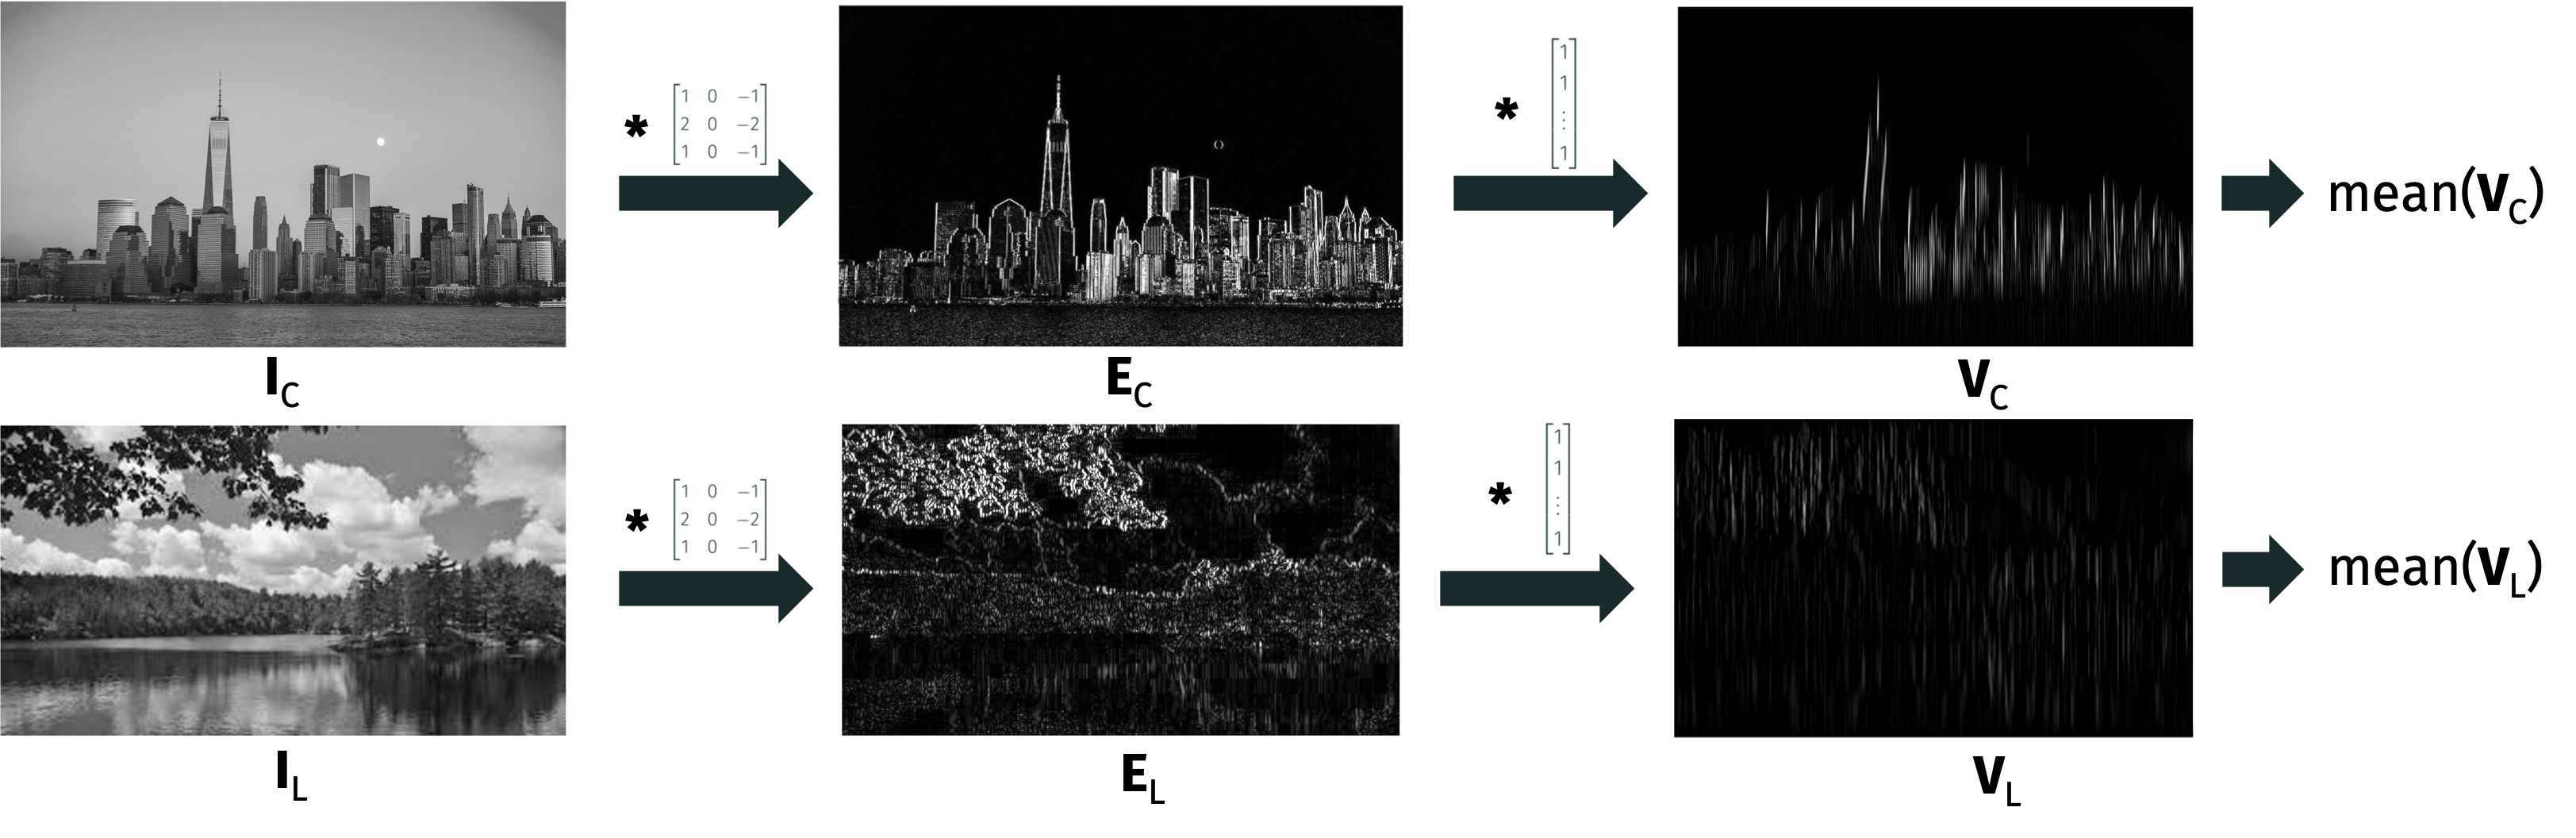
\includegraphics[width=\textwidth]{hier.png}
	
	$\texttt{mean}(\bv{V}_C) = .062$ \hspace{1em} vs. $\texttt{mean}(\bv{V}_L) = .054$
	
	$\texttt{mean}(\bv{V}_C\cdot \bv{V}_C) = .042$ \hspace{1em} vs. $\texttt{mean}(\bv{V}_L\cdot \bv{V}_L) = .018$
	\end{center}
	The image with highest average response to (edge detector) + (vertical pattern) is the city scape. 
	
	$\text{mean}(\bv{V})$ is an \emph{extracted scalar feature} which could be used for classifying cityscapes from landscapes using a linear classifier.
	
\end{frame}

	\begin{frame}
	\frametitle{hierarchical convolutional features}
	\begin{center}
	\textbf{Hierarchical combinations of simple convolution filters are \emph{very powerful} for understanding images.}
	\end{center}

In particular, \emph{edge detection} seems like a critical first step.

	\begin{center}
	\alert{\textbf{Lots of evidence from biology.}}
	\end{center}

	\end{frame}

	\begin{frame}
	\frametitle{visual system}
	\small
	Light comes into the eye through the lens and is detected by an array of photosensitive cells in the \textbf{retina}. 
	\begin{center}
		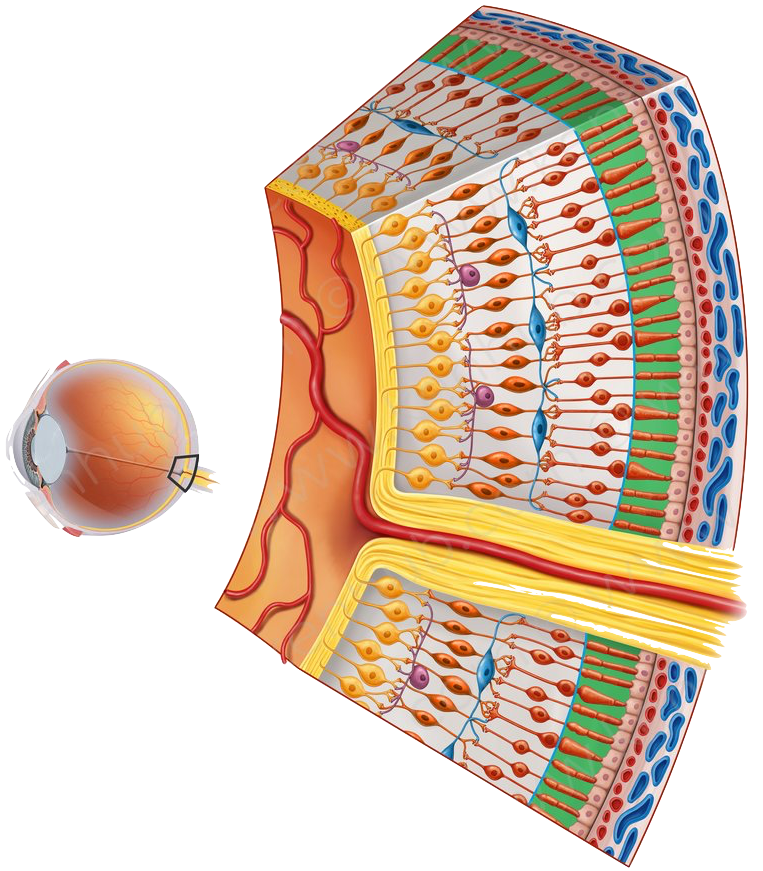
\includegraphics[width=.27\textwidth]{retina.png} \hspace{4em} 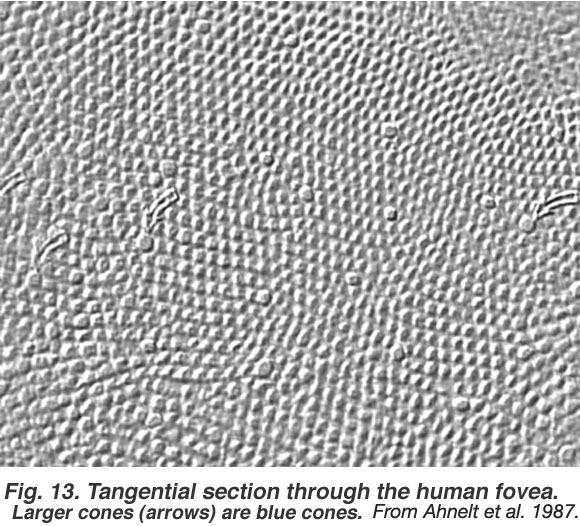
\includegraphics[width=.29\textwidth]{retina_micro.jpeg}
		
		\textbf{Rod} cells are sensitive to all light, larger \textbf{cone} cells are sensitive to specific colors. We have three types of cones:
		
			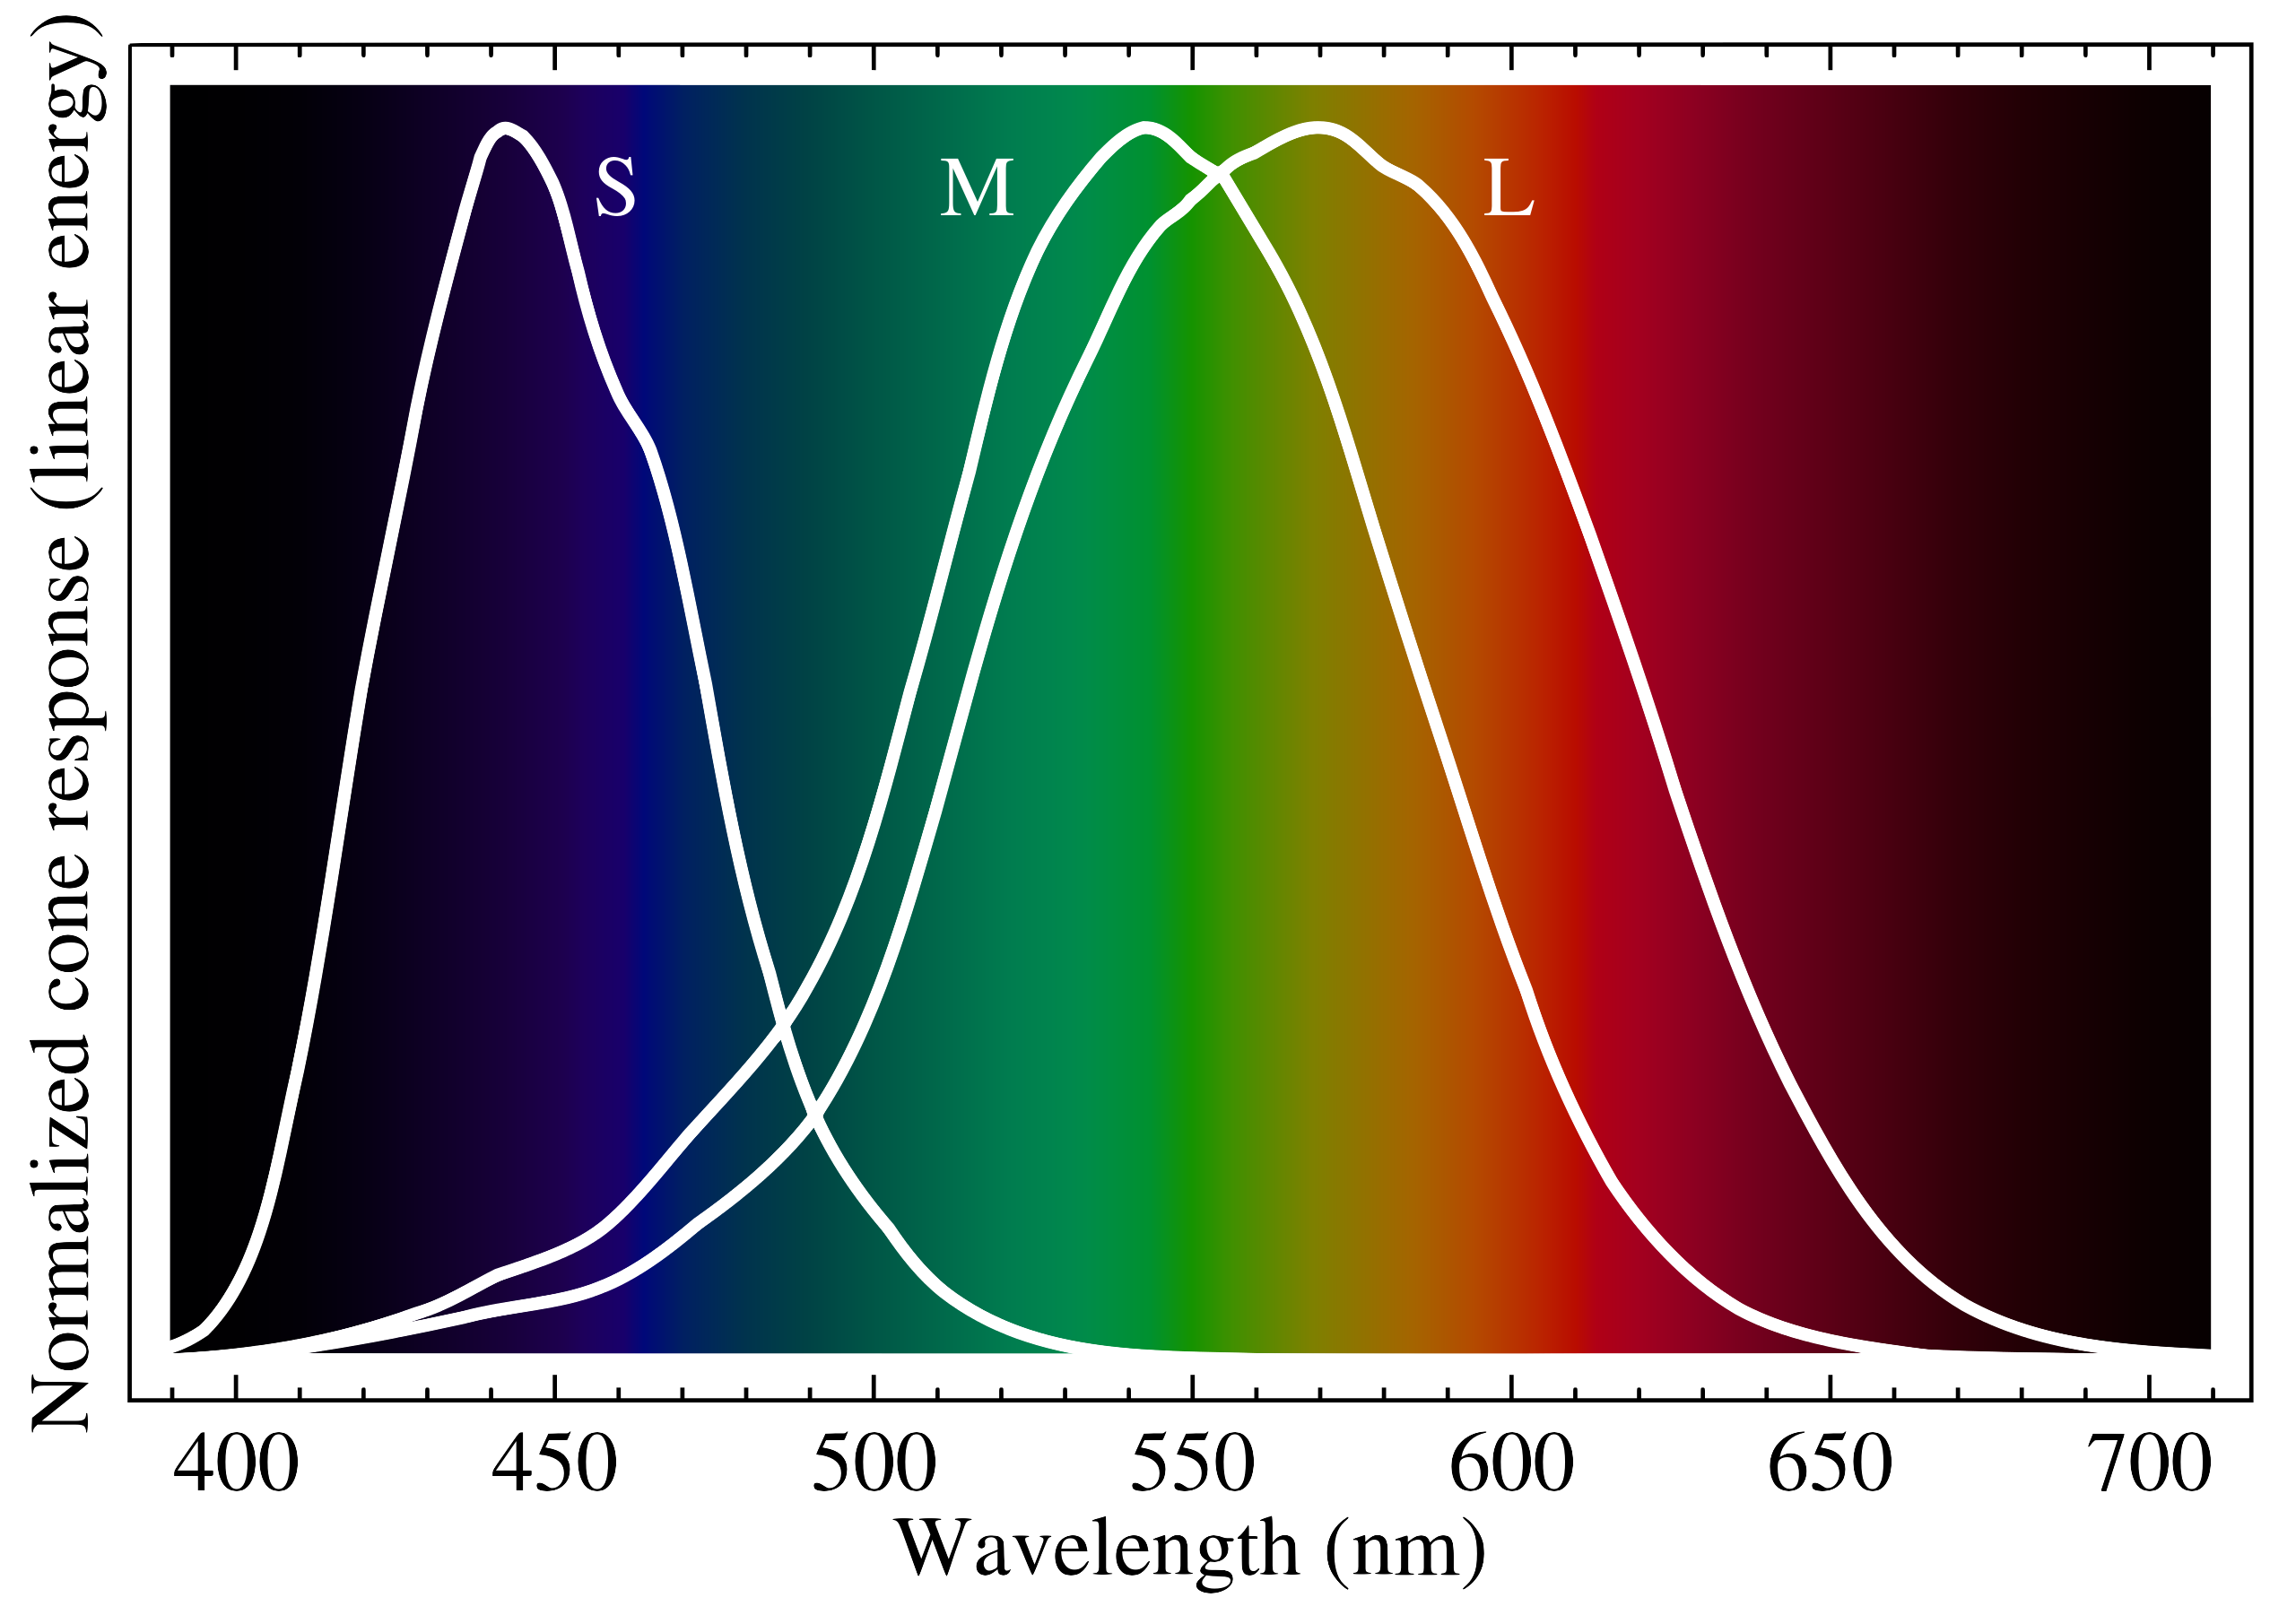
\includegraphics[width=.3\textwidth]{cone_response.png}
	\end{center}
\end{frame}

	\begin{frame}
	\frametitle{visual system}
	\small
	Signal passes from the retina to the primary (V1) visual cortex, which has neurons that connect to higher level parts of the brain.
	\begin{center}
			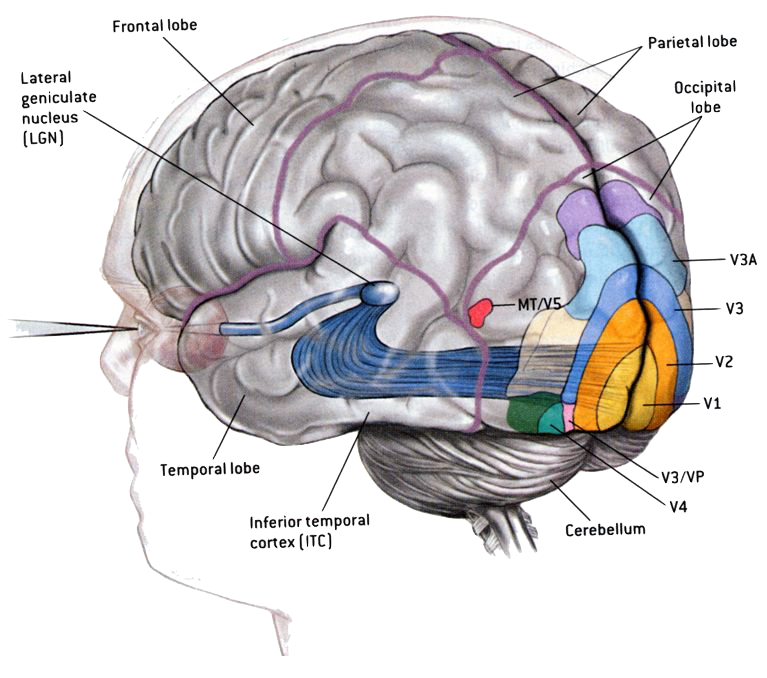
\includegraphics[width=.5\textwidth]{cortex.png}
			
			\textbf{What sort of processing happens in the primary cortex?} 
				
				\textbf{\alert{Lots of edge detection!}}
	\end{center}

	
	\end{frame}

	\begin{frame}
	\frametitle{edge detectors in cats}
	\small
	Huber + Wiesel, 1959: ``Receptive fields of single neurones in the cat's striate cortex.'' Won Nobel prize in 1981.
	\vspace{-.5em}
		\begin{center}
		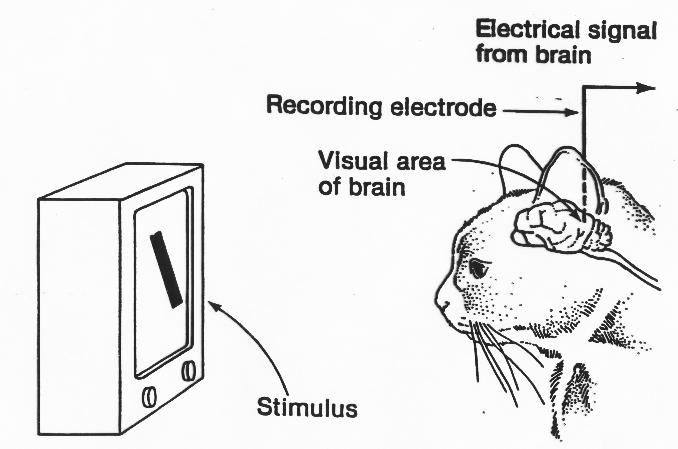
\includegraphics[width=.5\textwidth]{cat_experiment.jpg}
	\end{center}
	Different neurons fire when the cat is presented with stimuli at different angles. Cool video at \url{https://www.youtube.com/watch?v=OGxVfKJqX5E}.
	
	"What the Frog's Eye Tells the Frog's Brain", Lettvin et al. 1959. Found explicit edge detection circuits in a frogs visual cortex.
	\end{frame}

	\begin{frame}
	\frametitle{explicit feature engineering}
	State of the art until $\sim 10$ years ago:
	\begin{itemize}
		\item Convolve image with edge detection filters at many different angles.
		\item Hand engineer features based on the responses. 
		\item \textbf{SIFT} and \textbf{HOG} features were especially popular. 
	\end{itemize}
\begin{center}
	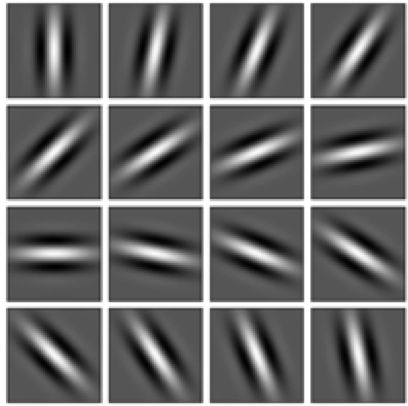
\includegraphics[width=.3\textwidth]{filter_bank.png}
\end{center}
	\end{frame}

	\begin{frame}
	\frametitle{convolutional neural networks}
	\small
	\textbf{Neural network approach:} Learn the parameters of the convolution filters based on training data. 
	\begin{center}
		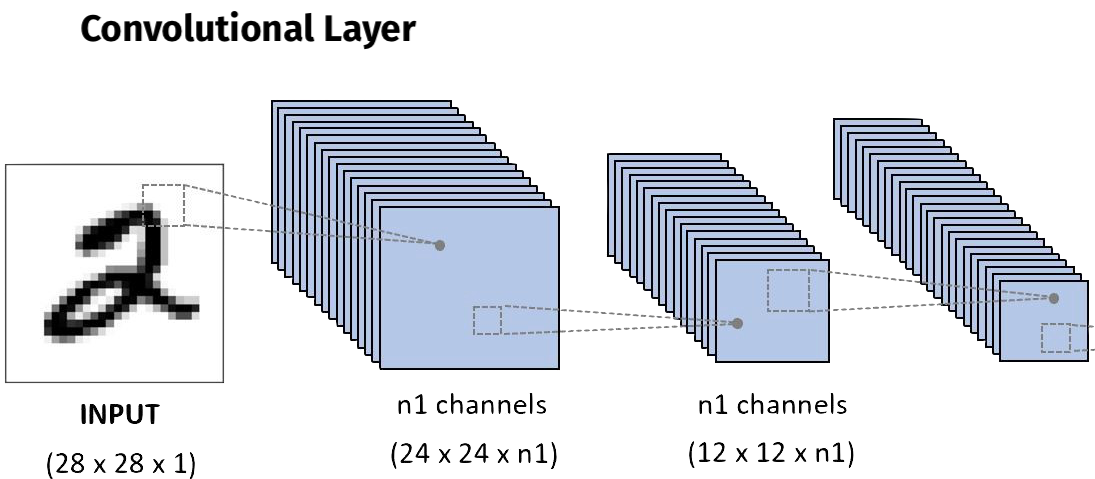
\includegraphics[width=.7\textwidth]{conv_net1.png}
	\end{center}
	First convolutional layer involves $n1$ convolution filters $\bv{W}_1, \ldots, \bv{W}_{n1}$. Each is small, e.g. $5\times 5$. Every entry in $\bv{W}_i$ is a free parameter: $\sim 25\cdot n1$ parameters to learn. 
	
	Produces $n1$ matrices of hidden variables: i.e. a tensor with depth $n1$.
	\end{frame}

	\begin{frame}
	\frametitle{convolutional neural networks}
	\small
	A fully connected layer that extracts the same feature would require $(28\cdot28\cdot24\cdot 24)\cdot n1 = \alert{451,584\cdot n1}$ parameters. 
	
	By ``baking in'' knowledge about what type of features matter, we greatly simply the network.

	\begin{center}
		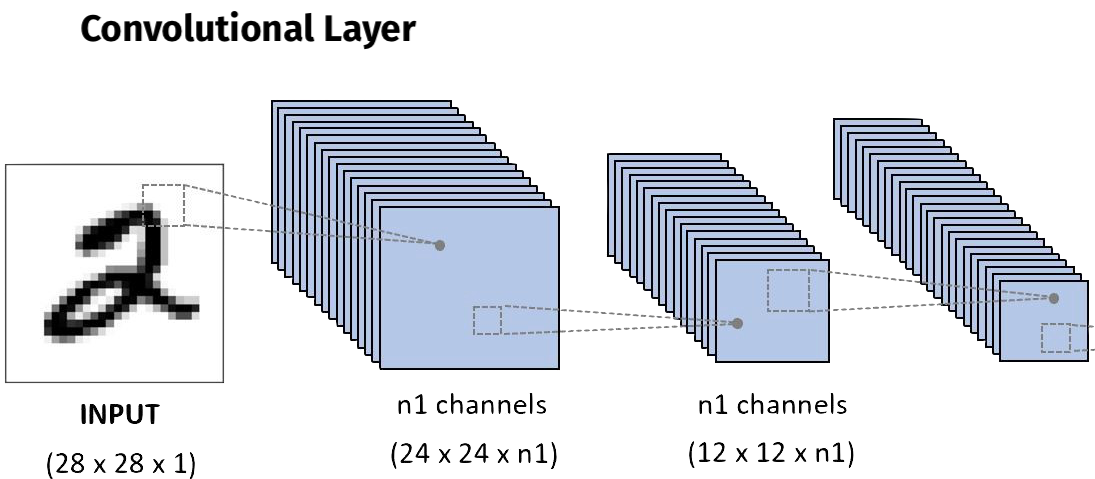
\includegraphics[width=.7\textwidth]{conv_net1.png}
	\end{center}
	Each of the $n1$ ouputs is typically processed with a \textbf{non-linearity}. Most commonly a Rectified Linear Unity (ReLU): $x = \max(\bar{x},0)$. 
\end{frame}

	\begin{frame}
	\frametitle{pooling and downsampling}
	Convolution + non-linearity are typically followed by a layer which performs \textbf{pooling + down-sampling}.
	\begin{center}
		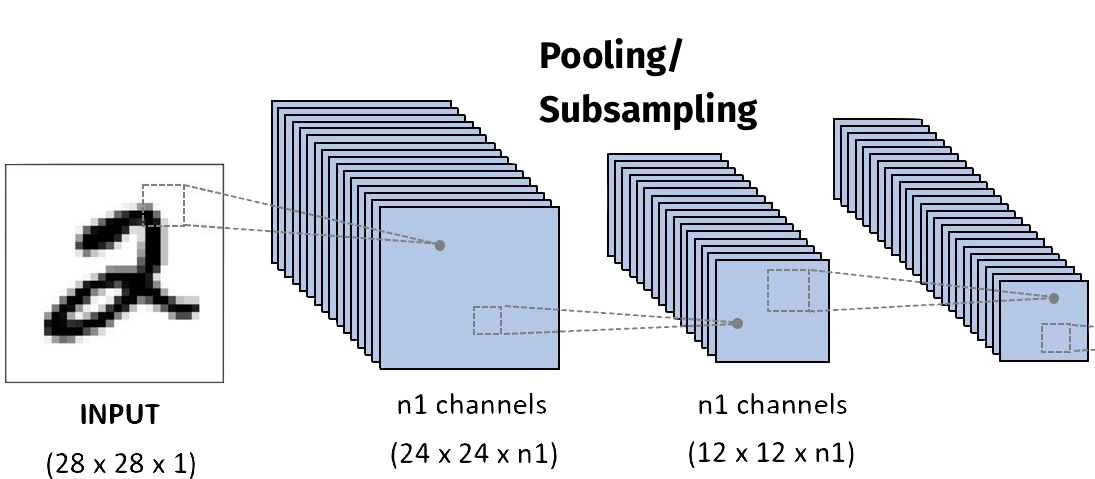
\includegraphics[width=.7\textwidth]{conv_net2.png}
	\end{center}
	\textbf{Most common approach is \alert{max-pooling}}.
	\end{frame}

	\begin{frame}
	\frametitle{pooling and downsampling}
	Convolution + non-linearity are typically followed by a layer which performs \textbf{pooling + down-sampling}.
	\begin{center}
		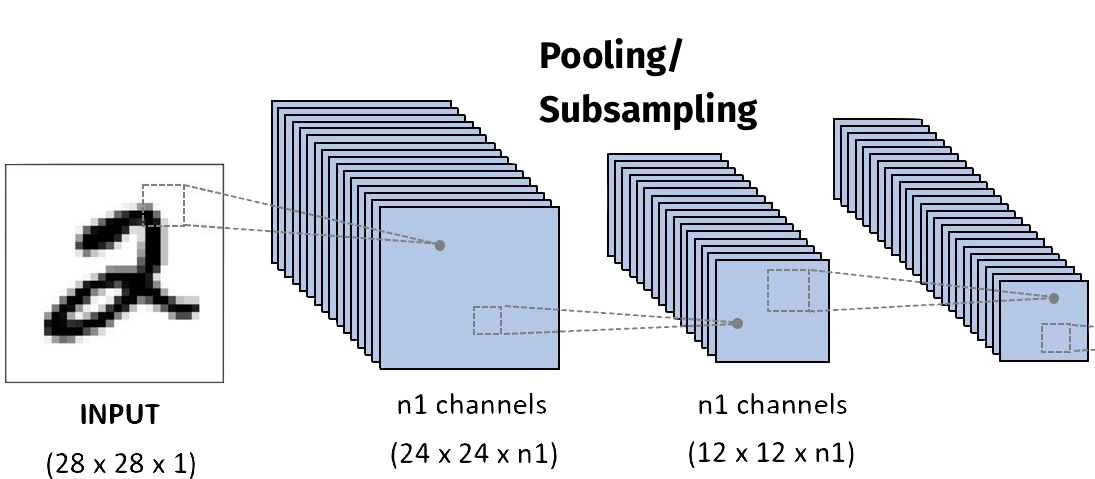
\includegraphics[width=.7\textwidth]{conv_net2.png}
		
		\textbf{Most common approach is \alert{max-pooling}}.
	\end{center}
	\end{frame}

	\begin{frame}
	\frametitle{pooling and downsampling}
	\small
	\begin{columns}
		\begin{column}{.5\textwidth}
			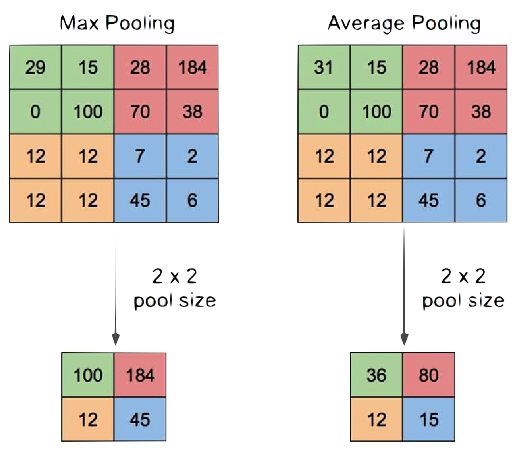
\includegraphics[width=\textwidth]{pooling_basic.png}
		\end{column}
	\begin{column}{.5\textwidth}
		\begin{itemize}
			\item Reduces number of variables, helps prevent over-fitting and speed up training.
			\item Helps ``smooth'' result of convolutional filters.
			\item Improves shift-invariance.
		\end{itemize}
	\end{column}
	\end{columns}
	\begin{center}
		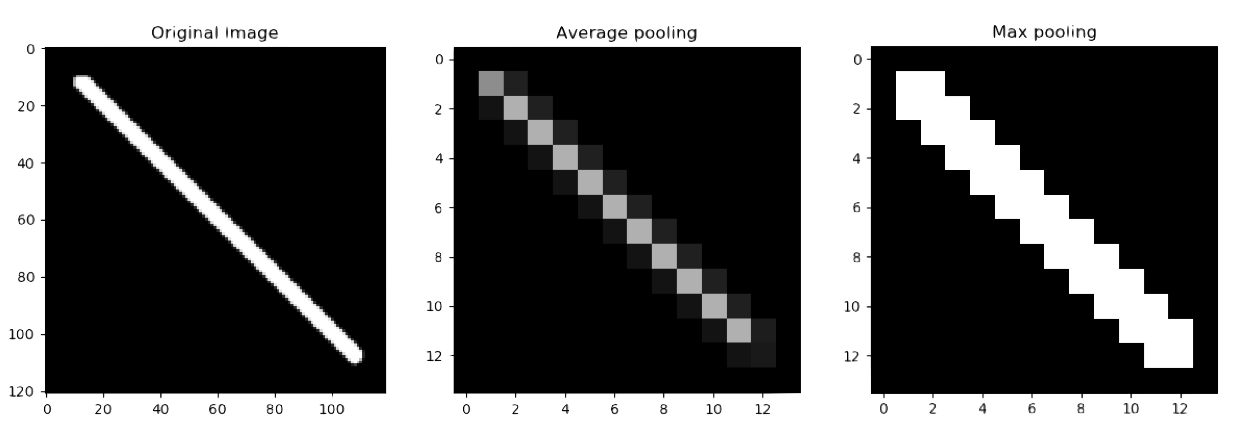
\includegraphics[width=.6\textwidth]{effect_of_max_pooling.png}
	\end{center}
	\end{frame}

	\begin{frame}
	\frametitle{pooling and downsampling}
	Many possible variations on standard 2x2 max-pooling.
	\begin{center}
		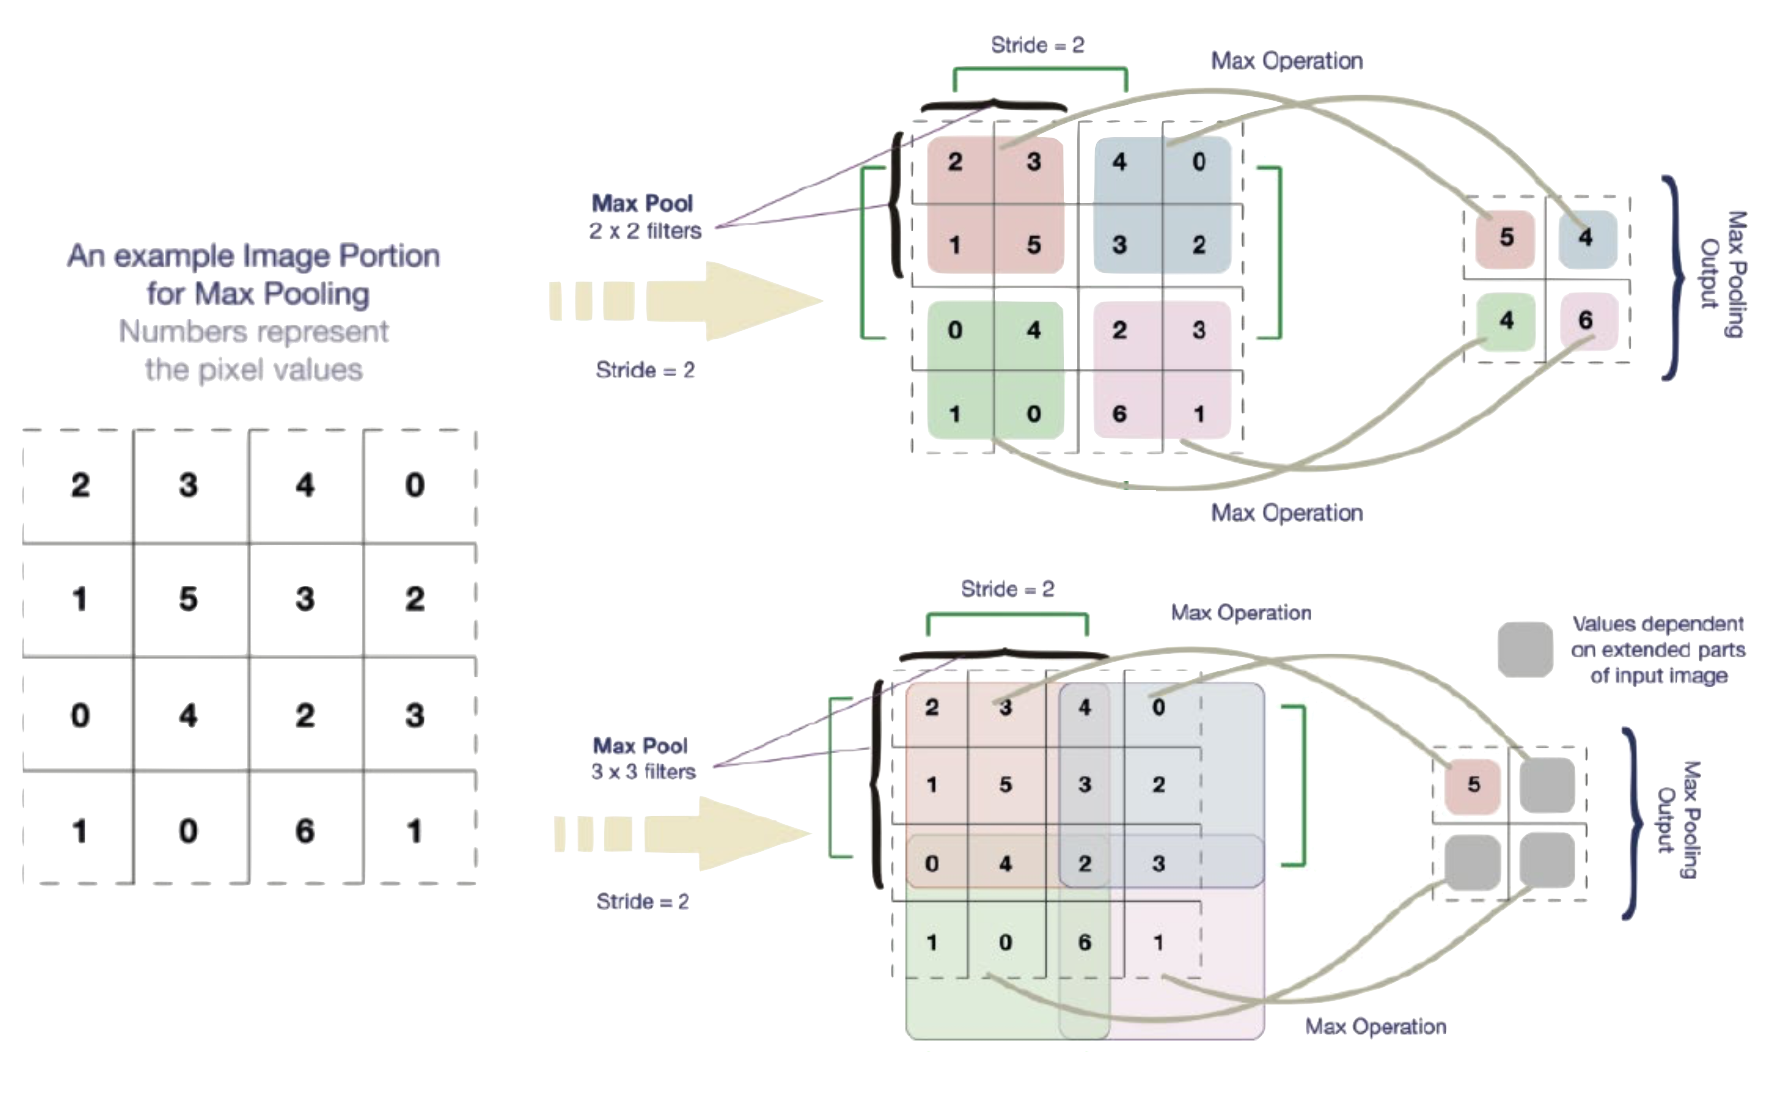
\includegraphics[width=\textwidth]{pooling_advanced.png}
	\end{center}
	\end{frame}

	\begin{frame}
	\frametitle{overall network architecture}
	\begin{center}
		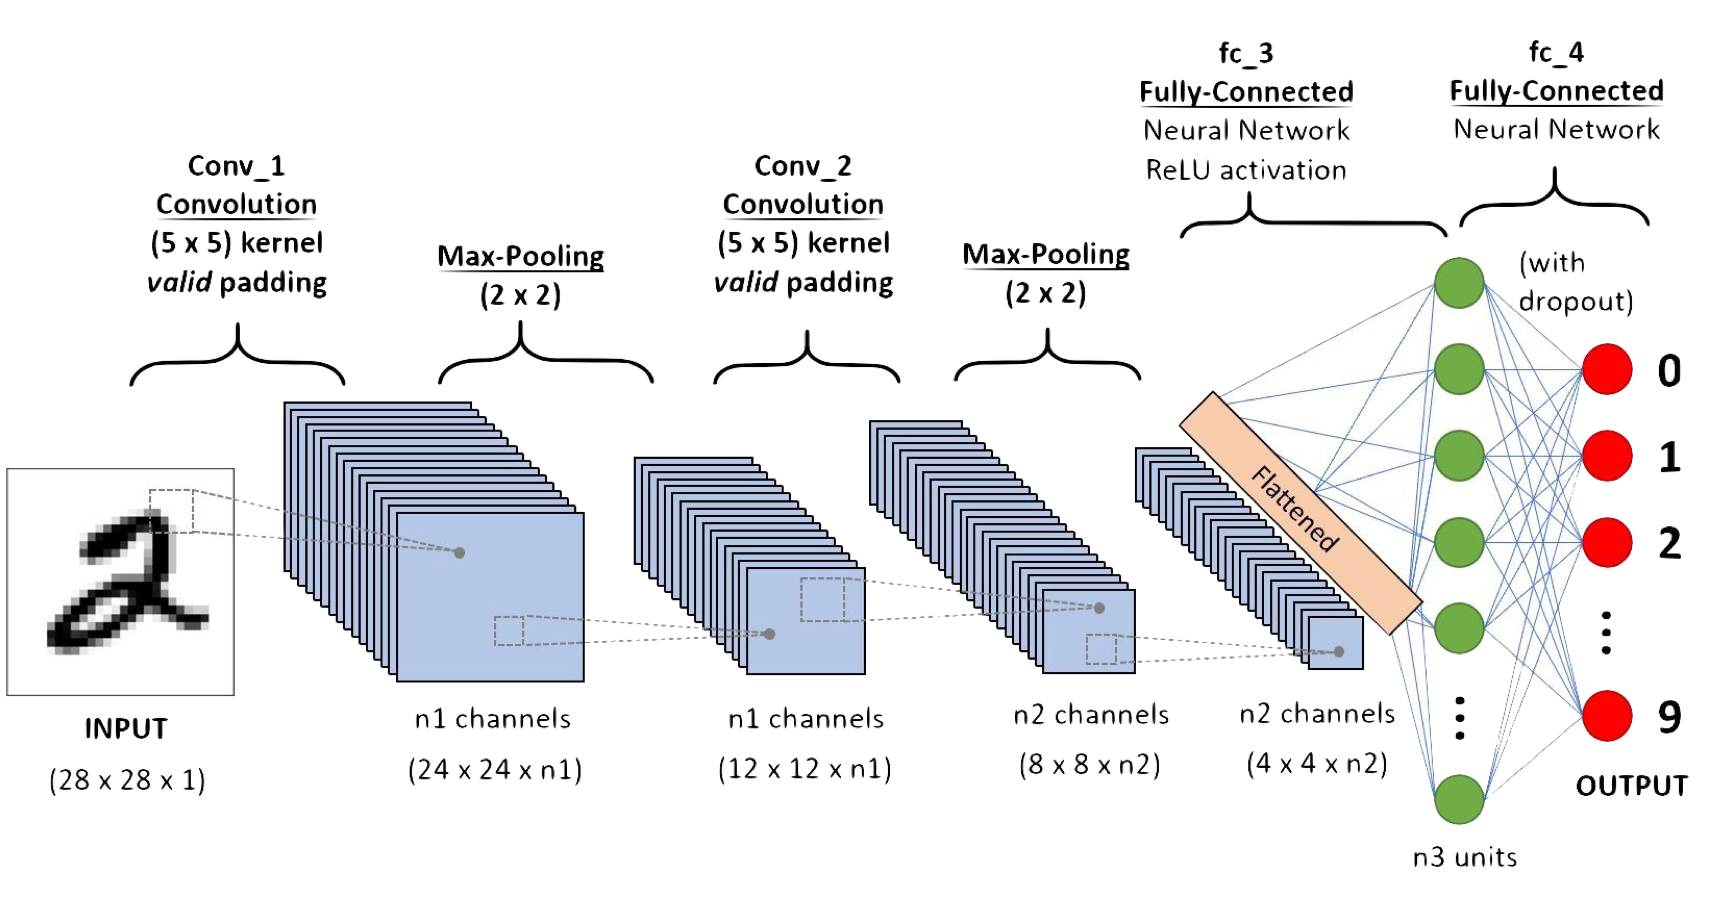
\includegraphics[width=\textwidth]{conv_net.png}
		
		Each layer contains a 3D tensor of variables. Last few layers are standard fully connected layers. 
	\end{center}
	\end{frame}


\begin{frame}
	\frametitle{understanding layers}
	\small
	What type of convolutional filters do we learn from gradient descent? \textbf{Lots of edge detectors in the first layer!}
	\begin{center}
		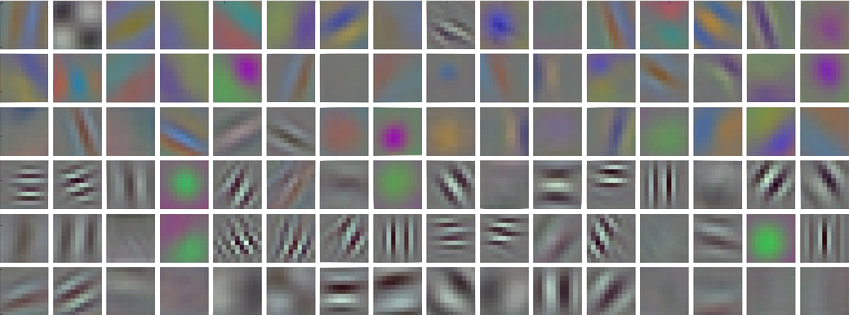
\includegraphics[width=.6\textwidth]{first_layer.png}
	\end{center}
Other layers are harder to understand... but the hypothesis is that hidden variables later in the network encode for ``higher level features'':
	\begin{center}
	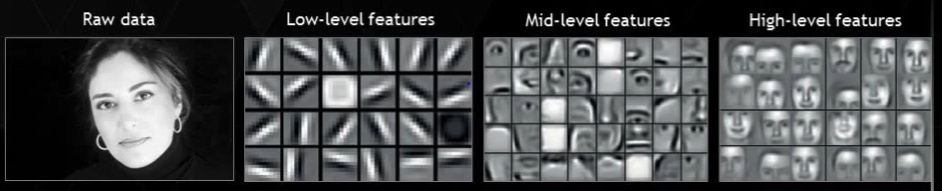
\includegraphics[width=\textwidth]{mid_level.png}
	\end{center}
\end{frame}

\begin{frame}
	\frametitle{understanding layers}\small
	\textbf{Technique to probe later neurons:} Use optimization to find images that most strongly ``activate'' a given neuron deep in the network. 
	
	\begin{center}
		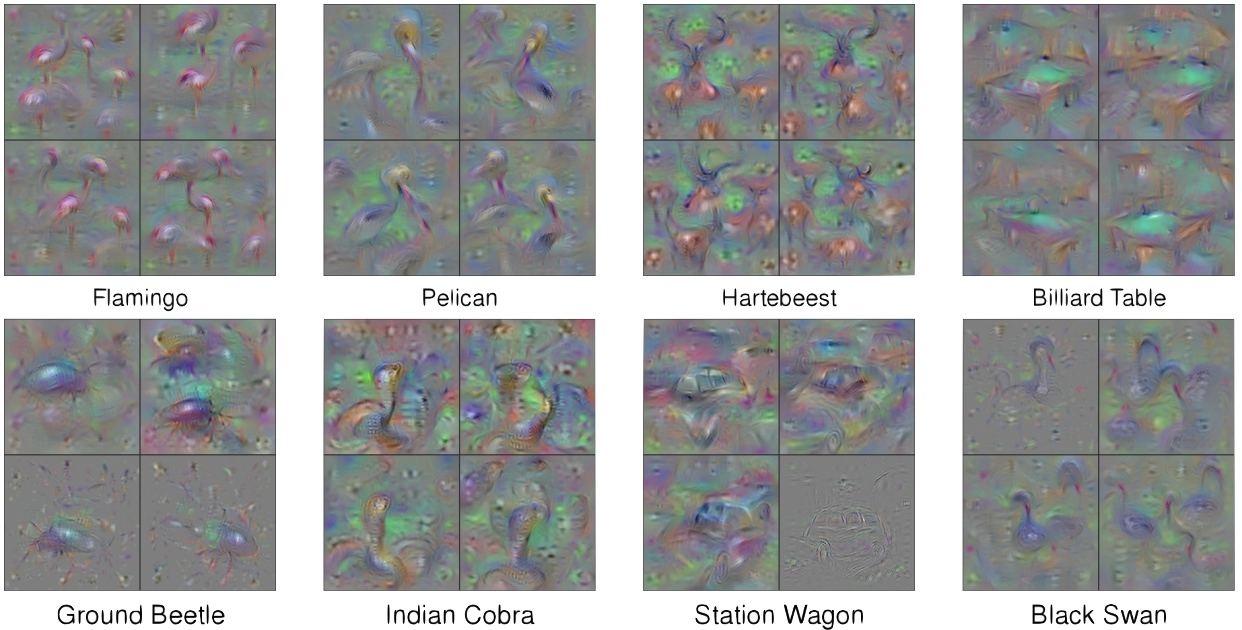
\includegraphics[width=\textwidth]{clune_paper.png}
	\end{center}
	\footnotesize{``Understanding Neural Networks Through Deep Visualization'', Yosinski et al.}
\end{frame}

\begin{frame}
	\frametitle{tricks of the trade}\small
	Beyond techinques discussed for general neural nets (back-prop, batch gradient descent, adaptive learning rates) training convolutional networks requires a lot of ``tricks''. 
	\begin{itemize}
		\item Batch normalization (accelerate training).
		\item Dropout (prevent over-fitting)
		\item Residual connections (accelerate training, allow for more depth -- 100s of layers).
	\end{itemize}
\begin{center}
	\textbf{ And convolutional networks require \alert{lots of training data.}}
\end{center}
\end{frame}

\begin{frame}
	\frametitle{transfer learning}
	\small
	What if you want to apply deep convolutional networks to a problem where you don't have a lot of data?
	
	\textbf{Idea behind \emph{transfer learning}}: features transformations learned when training a classifier on e.g. Imagenet are often useful in other problems, even with different inputs, classes, etc. 
	\begin{center}
		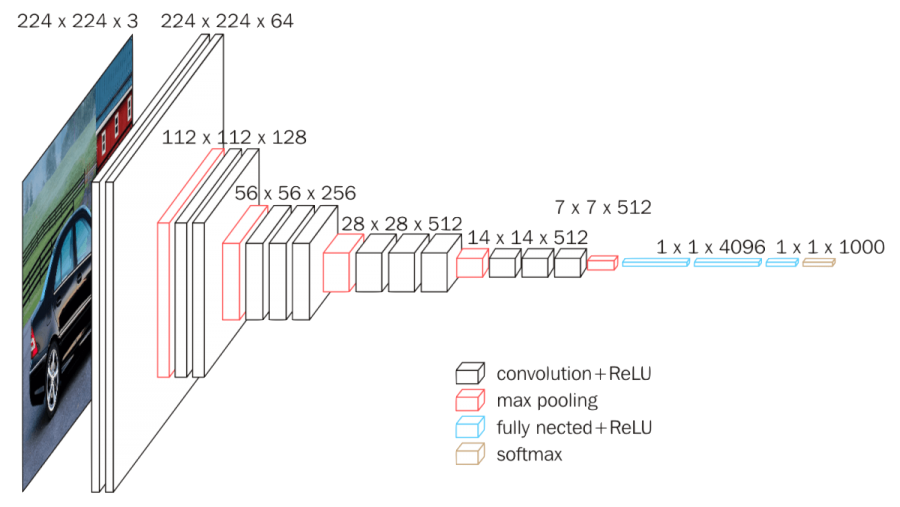
\includegraphics[width=.7\textwidth]{vgg.png}
	\end{center}
\end{frame}

\begin{frame}
	\frametitle{transfer learning}
	\begin{itemize}
		\item Download state of the art pre-trained network (Alexnet, VGG, Inception, etc.)
		\item Chop off classification layer. 
		\item Use first part of network as feature extractor. 
		\item Solve classification problem using more scalable methods: kernel SVM, logistic regression, shallow fully connected net, etc.
	\end{itemize}
	\textbf{Very easy to do in Tensorflow/Keras}. Many pre-trained networks are made available. 
\end{frame}

\begin{frame}
	\frametitle{demos}
	\textbf{Two demos to be released shortly:}
			\begin{center}
	\begin{itemize}
		\item Classification of CIFAR-10 dataset using 2 layer neural nets in Keras. You will likely want to use Google Collab to access a GPU.
		
		\vspace{.5em}
	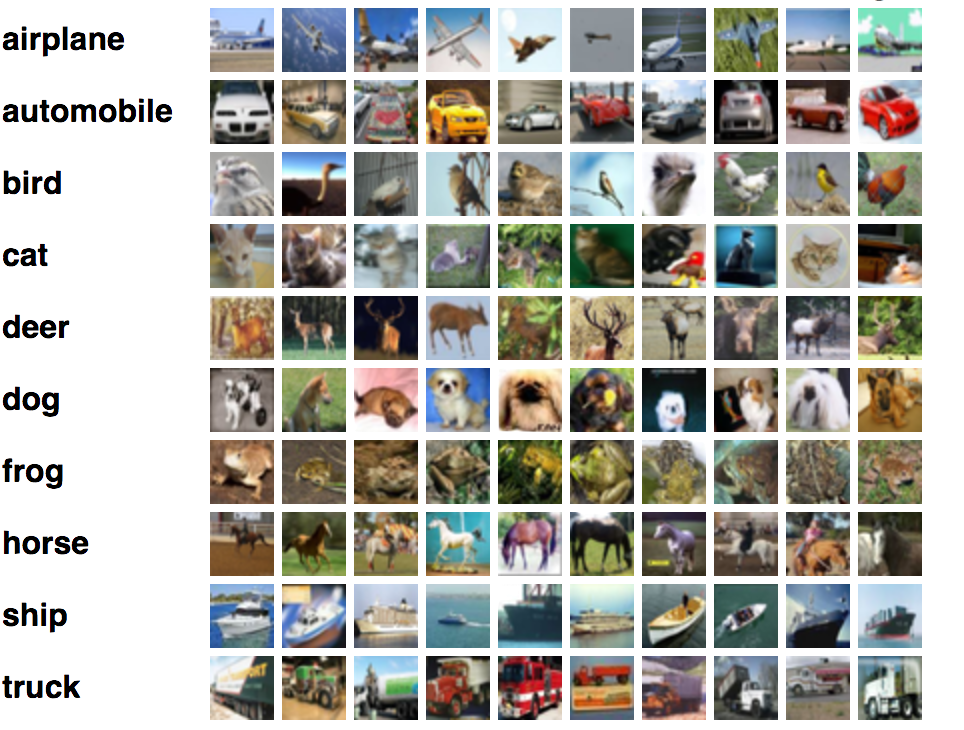
\includegraphics[width=.4\textwidth]{cifar10.png}
		
		\item Transfer learning in Keras.
	\end{itemize}
\end{center}
	
\end{frame}

\end{document} 



